\documentclass[11pt]{tg_usta}
% Informe final del Taller de RAG - Procesamiento de Lenguaje Natural
% Pontificia Universidad Javeriana, Maestria en Inteligencia Artificial

\usepackage{float}
\usepackage{graphicx}
\usepackage{anysize}
\marginsize{1in}{1in}{1in}{1in}
\usepackage{amsmath,amssymb}
\usepackage{url}
\usepackage{array}
\usepackage{booktabs}
\usepackage{multirow}
\usepackage[T1]{fontenc}
\usepackage[utf8]{inputenc}
\usepackage{tikz}
\usepackage{subcaption}

\renewcommand{\tablename}{Tabla}
\renewcommand{\figurename}{Figura}
\graphicspath{{../figuras/}}

\begin{document}

\title[maintitle = Asistente RAG reproducible sobre prensa y Bluesky con Milvus y modelos locales pequeños,
       shorttitle = RAG reproducible con Milvus y modelos locales,
       secondtitle = Taller de RAG - Procesamiento de Lenguaje Natural]

\begin{authors}[Rivera, Carrillo, Garnica \& Prieto]

\author[affiliation = PUJ,
        firstname = Erika Valeria,
        surname = Rivera Jimenez,
        email = riveraev@javeriana.edu.co]

\author[affiliation = PUJ,
        firstname = Julian Guillermo,
        surname = Carrillo Meneses,
        email = carrillojuliang@javeriana.edu.co]

\author[affiliation = PUJ,
        firstname = Carlos Andres,
        surname = Garnica Salazar,
        email = carlos\_garnicas@javeriana.edu.co]

\author[affiliation = PUJ,
        firstname = Oscar Andres,
        surname = Prieto Moreno,
        email = o-prieto@javeriana.edu.co]

\end{authors}

\begin{mainabstract}
Se construyó un asistente de recuperación aumentada sobre 169.248 documentos de prensa y Bluesky, con Milvus como único motor vectorial y cuatro modelos generativos locales de 1 a 3 mil millones de parámetros servidos por Ollama. El sistema completo se levanta con un único archivo de Docker Compose. La evaluación se apoya en un gold de 43 preguntas revisadas por dos anotadores y en una ampliación de 17 documentos añadidos por consenso entre ambos (kappa 0,626). Se compararon cuatro variantes de limpieza, dos estrategias de segmentación, tres tamaños de contexto y tres codificadores sobre un piloto estratificado de 2.000 documentos; después se repitió la medición sobre el corpus completo. El hallazgo principal es que el piloto sobreestima la recuperación: con el mismo codificador, el mismo índice y las mismas 38 preguntas respondibles, Recall@10 cae de 0,947 a 0,684 y nDCG@10 de 0,909 a 0,594 al pasar de 1.932 a 161.868 documentos indexados con e5-base. La latencia no explica la caída, que es de ordenamiento. BM25 sparse recupera 0,763 y bge-m3 0,842; el ajuste de ef y la fusión con BM25 llevan el Recall@10 a 0,895. Con el gold ampliado, el recuperador final (bge-m3, ef=800, sin fusión) alcanza Recall@10 de 0,921, nDCG@10 de 0,827 y P@1 de 0,737. Un cross-encoder sobre el top-50 mejora el orden (P@1 de 0,474 a 0,632 y nDCG@10 de 0,594 a 0,661) pero no la cobertura y añade 3,1 s por consulta, así que no se adopta para la demostración. Ninguna ablación de limpieza, segmentación o tamaño de contexto alcanza significancia estadística con el gold actual. La anotación humana de 72 respuestas, con dos anotadores y kappa de 0,95 en corrección, elige gemma2:2b, que supera en corrección y citas a qwen2.5:1.5b. La hipótesis H1 se refuta.
\keywords{recuperación aumentada, Milvus, recuperación densa, bge-m3, evaluación de recuperación, reranking, modelos locales}
\end{mainabstract}

\section{Problema y motivación}

Un asistente de recuperación aumentada (RAG) combina un recuperador que selecciona evidencia de una colección con un modelo de lenguaje que redacta una respuesta a partir de esa evidencia \cite{lewis2020rag}. La calidad final depende de dos eslabones que fallan de forma distinta: si el recuperador no trae el documento correcto, el generador no puede responder; si lo trae pero lo coloca tarde en el contexto, el modelo puede ignorarlo \cite{liu2024lost}. La literatura de recuperación muestra que el desempeño cae al cambiar de dominio y de idioma \cite{thakur2021beir,zhang2023miracl}, y que los codificadores multilingües se comparan en bancos como MTEB \cite{muennighoff2023mteb}. Este taller pedía construir ese sistema sobre un corpus real de prensa y redes sociales, con Milvus como único motor vectorial, modelos generativos locales y una evaluación que separara recuperación de generación.

El corpus del taller tiene las condiciones de un caso real y no las de un banco de pruebas: 169.248 documentos con ruido de crawler, duplicados exactos y casi duplicados, un campo de idioma que mezcla códigos ISO con locales, y un tercio de los textos truncados por el recolector. Esas condiciones obligan a decidir qué se limpia, qué se descarta y qué se declara como límite.

La pregunta que organiza el trabajo es doble. La primera parte es comparativa: con la misma evidencia recuperada, ¿qué modelo local pequeño ofrece el mejor equilibrio entre corrección, fidelidad, abstención, latencia y consumo de recursos? La segunda parte es metodológica: ¿las conclusiones obtenidas sobre una muestra pequeña se sostienen cuando el corpus crece dos órdenes de magnitud? La segunda pregunta no estaba en el enunciado original y surgió de un resultado que contradijo la expectativa inicial, que se reporta como hallazgo principal.

Las restricciones del taller acotan el espacio de soluciones. No se permiten API de pago, Milvus es el único motor vectorial, todo debe levantarse desde Docker Compose y la demostración corre en un equipo con una GPU AMD de 16 GB más un servidor con una GTX 1080. La consecuencia práctica es que el sistema tiene que funcionar con modelos de 1 a 3 mil millones de parámetros y con un codificador que quepa en CPU, porque la GPU local se reserva para la generación.

Las contribuciones del informe son cuatro. Primero, un pipeline reproducible de ingesta, indexación, consulta y evaluación, con artefactos crudos versionados y métricas calculadas desde esos artefactos. Segundo, una ablación pareada de cuatro variantes de limpieza con corrección de Bonferroni. Tercero, una medición de la degradación por escala entre el piloto y el corpus completo, que es el resultado central. Cuarto, la medición del costo y el beneficio de un cross-encoder sobre el corpus completo y una prueba acotada de resistencia a instrucciones inyectadas en los documentos.

\section{Hipótesis y preguntas de investigación}

El trabajo se organizó con cuatro hipótesis verificables. La Tabla~\ref{tab:hipotesis} las resume con la prueba asociada y el estado en que quedaron al cierre de este informe.

\begin{table}[htbp]
\centering
\footnotesize
\begin{tabular}{@{}p{0.7cm}p{6.1cm}p{4.3cm}p{3.4cm}@{}}
\toprule
 & Hipótesis & Prueba & Estado \\
\midrule
H1 & llama3.2:3b tendrá mayor fidelidad y corrección que qwen2.5:1.5b y gemma2:2b con la misma evidencia, a costa de latencia. & E4, 24 preguntas de prueba, 4 modelos, 3 repeticiones. & Refutada: ver E4. \\
\addlinespace
H2 & La limpieza conservadora mejora la recuperación frente al texto crudo. & Ablación V0 a V3, 30 preguntas, bootstrap pareado con Bonferroni. & No concluyente: ninguna diferencia de calidad excluye cero. \\
\addlinespace
H3 & El chunking por oraciones mejora el chunking fijo de 1.000 caracteres. & E1, 30 preguntas, mismas condiciones de índice. & No concluyente: nDCG $-0,071$ con IC $[-0,221;\,0,025]$. \\
\addlinespace
H4 & La recuperación medida en el piloto se mantiene al escalar al corpus completo. & E6, 38 preguntas respondibles, mismo codificador e índice. & Refutada: Recall@10 cae de 0,947 a 0,684. \\
\bottomrule
\end{tabular}
\caption{Hipótesis, prueba asociada y estado al cierre.}
\label{tab:hipotesis}
\end{table}

La distinción entre ``no concluyente'' y ``refutada'' importa. En H2 y H3 la estimación puntual favorece la alternativa adoptada, pero el intervalo de confianza de la diferencia contiene cero con 30 preguntas, así que no se declara superioridad. En H4 las dos colecciones se evaluaron con las mismas 38 preguntas y los intervalos de Recall@10 no se solapan ([0,904; 0,983] en el piloto frente a [0,605; 0,772] en el corpus completo), de modo que la caída no se atribuye al muestreo de preguntas.

\section{Datos y perfilado}

\subsection{Composición del corpus}

El archivo de trabajo tiene 169.248 filas, 34 columnas y 256,9 MB. La columna \texttt{document\_id} es única y no hay textos vacíos ni URLs nulas. La composición por colección se muestra en la Tabla~\ref{tab:composicion}: 104.578 documentos provienen de rastreo web y 64.670 de Bluesky.

\begin{table}[htbp]
\centering
\small
\begin{tabular}{lrr}
\toprule
Colección & Documentos & \% del total \\
\midrule
\texttt{url\_crawls} (prensa) & 104.578 & 61,8 \\
\texttt{bluesky\_posts} (redes) & 64.670 & 38,2 \\
\midrule
Total & 169.248 & 100,0 \\
\bottomrule
\end{tabular}
\caption{Composición del corpus por colección de origen.}
\label{tab:composicion}
\end{table}

El campo \texttt{source\_type} no sirve como etiqueta semántica: 99.326 filas lo tienen nulo, 64.670 valen \texttt{social\_post} y solo 5.252 valen \texttt{news\_article}. La distribución por dominio confirma el peso de las fuentes: bsky.app aporta 64.670 documentos, infobae 19.766, eltiempo 12.229, theguardian 7.216 y elespectador 5.456. La consecuencia para el informe es que el corpus no representa la conversación pública en español: Bluesky llega casi todo en inglés y la prensa está dominada por cuatro cabeceras.

\subsection{Duplicados}

Hay 14.771 filas que comparten el mismo \texttt{text\_sha256}, agrupadas en 4.434 grupos, con un máximo de 839 copias de un mismo texto. Los documentos que forman parte de un grupo duplicado se reparten entre las dos colecciones (9.972 en Bluesky y 9.233 en prensa). El archivo no se modifica: la deduplicación se hace en la recuperación, comparando el hash del chunk antes de armar el contexto, tal como se decidió en el ADR-008. La razón es de trazabilidad: borrar filas en la ingesta perdería la procedencia y haría imposible auditar qué se descartó.

\subsection{Longitud y truncamiento}

La Tabla~\ref{tab:longitud} resume la distribución de longitud. La media es de 473 palabras y 2.977 caracteres, pero la mediana baja a 371 palabras y 2.367 caracteres, señal de una cola larga: el percentil 99 llega a 2.420 palabras y el máximo a 58.181 palabras, equivalentes a 363.528 caracteres. Ese documento extremo produce cientos de chunks y obliga a controlar el tamaño de lote en la ingesta.

\begin{table}[htbp]
\centering
\small
\begin{tabular}{lrrrrr}
\toprule
Unidad & Media & Mediana & p90 & p99 & Máximo \\
\midrule
Palabras & 473 & 371 & 1.010 & 2.420 & 58.181 \\
Caracteres & 2.977 & 2.367 & 6.361 & 15.142 & 363.528 \\
\bottomrule
\end{tabular}
\caption{Distribución de longitud de los 169.248 documentos.}
\label{tab:longitud}
\end{table}

La textometría sobre la muestra de 5.000 documentos cuantifica el truncamiento: 32,7\,\% de los documentos termina a mitad de frase o en un corte del recolector (33,5\,\% en el piloto). La limpieza no puede recuperar ese texto. Es una limitación del corpus que se declara en la Sección~\ref{sec:limitaciones} y que acota lo que cualquier recuperador puede lograr.

\subsection{Fechas e idioma}

El rango declarado de fechas va de 2008 a 2026, pero la distribución real se concentra en 2024 (171 documentos), 2025 (1.592) y 2026 (3.515). El resto son fechas sueltas de años anteriores. El filtro temporal solo es fiable en el tramo 2024 a 2026 y así se documenta en la interfaz.

El campo \texttt{language} mezcla códigos ISO con locales y variantes de mayúsculas: conviven \texttt{en}, \texttt{en-global}, \texttt{en-gb}, \texttt{en-us} y \texttt{en-US}, y lo mismo ocurre con el español. Tras normalizar, el corpus queda en 82.682 documentos en inglés, 66.910 en español y 13.140 sin idioma declarado. El húngaro aparece con 4.108 documentos en el campo crudo, un volumen que no se corresponde con el resto de la distribución y que se excluye del filtro de idioma hasta revisarlo. La normalización se hace al vuelo en la ingesta y el archivo original no se toca.

\subsection{Ruido del crawler}

El crawler dejó páginas de error dentro del corpus. La misma página con los mensajes ``Haz excedido el máximo de peticiones'' y ``Error 505'' aparece en 7.378 documentos, el 4,36\,\% del total, todos en la colección de prensa. En el conjunto de humo esos textos casi idénticos dominaban el top-10 de cualquier consulta, porque su similitud entre sí es mayor que la de cualquier documento relevante. El filtro de calidad los descarta en la ingesta y los cuenta en el resumen. El porcentaje de documentos con al menos un patrón de ruido (peticiones, error 505, cookies, inicio de sesión) llega al 5,3\,\%, pero el filtro solo elimina los marcadores fuertes de error y no las menciones legítimas de cookies.

\subsection{Textometría}

La textometría se calculó sobre dos muestras: los 2.000 documentos del piloto y 5.000 documentos estratificados del resto del corpus, con semilla 42. La Tabla~\ref{tab:textometria} compara los indicadores.

\begin{table}[htbp]
\centering
\footnotesize
\begin{tabular}{lrr}
\toprule
Indicador & Piloto (2.000) & Muestra (5.000) \\
\midrule
Tipos por documento (mediana) & 188 & 188 \\
TTR mediana & 0,579 & 0,570 \\
Hapax / tipos (mediana) & 0,773 & 0,770 \\
Guiraud (mediana) & 10,04 & 10,13 \\
Caracteres por documento (mediana) & 2.317 & 2.353 \\
Caracteres p99 & 14.979 & 15.498 \\
Documentos truncados & 33,5\,\% & 32,7\,\% \\
Documentos con URL & 9,3\,\% & 9,9\,\% \\
Documentos con correo electrónico & 1,8\,\% & 1,3\,\% \\
Documentos con emojis & 12,4\,\% & 12,1\,\% \\
Documentos con navegación & 3,4\,\% & 3,3\,\% \\
Documentos con boilerplate & 3,4\,\% & 4,5\,\% \\
Documentos con near-duplicate (SimHash) & 4,25\,\% & 4,72\,\% \\
Grupos de near-duplicates & 26 & 53 \\
Grupo más grande & 12 & 32 \\
\bottomrule
\end{tabular}
\caption{Indicadores de textometría en el piloto y en la muestra del resto del corpus.}
\label{tab:textometria}
\end{table}

Tres lecturas se desprenden de la tabla. La primera es que el piloto es representativo en longitud y riqueza léxica: la mediana de tipos por documento es idéntica (188) y el TTR difiere en nueve milésimas. La segunda es que el ruido no es solo hash exacto: SimHash con distancia de Hamming menor o igual a 3 encuentra grupos de hasta 32 documentos que el hash exacto no captura, y esa es la razón por la que V3 deduplica por chunk y no por documento. La tercera es que los términos exclusivos de prensa están dominados por boilerplate (``publicidad'', ``información'', ``además''), lo que anticipa que la normalización conservadora puede ayudar sin necesidad de diccionarios.

La Figura~\ref{fig:perfil} presenta el perfil del corpus y la Figura~\ref{fig:textometria} los indicadores textométricos.

\begin{figure}[htbp]
\centering
\begin{subfigure}[b]{0.48\textwidth}
\centering
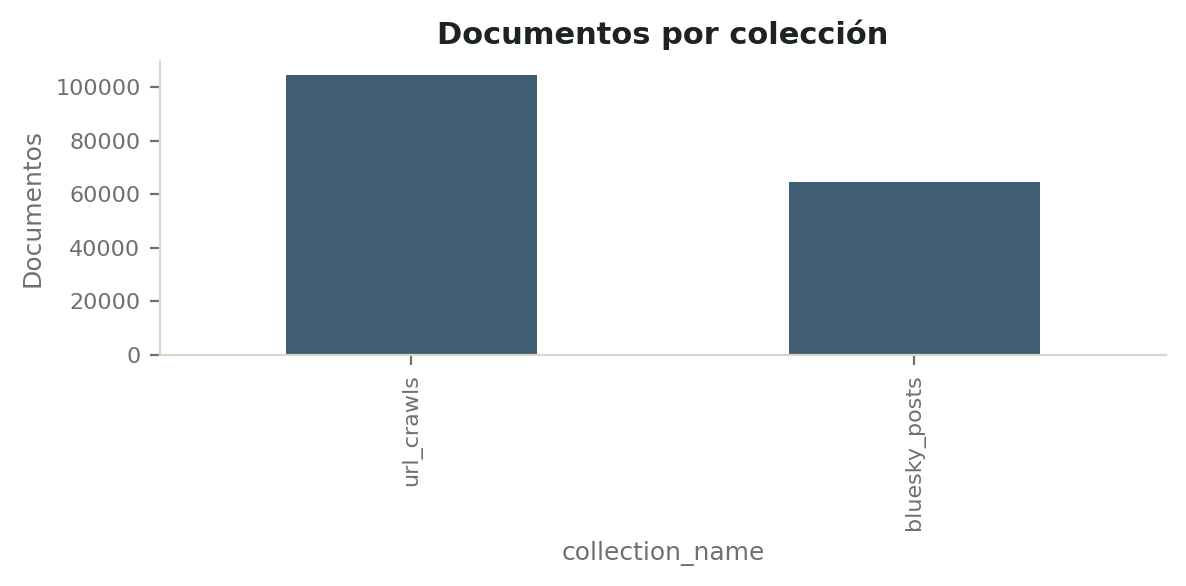
\includegraphics[width=\textwidth]{perfil_colecciones.png}
\caption{Documentos por colección.}
\label{fig:perfil-colecciones}
\end{subfigure}\hfill
\begin{subfigure}[b]{0.48\textwidth}
\centering
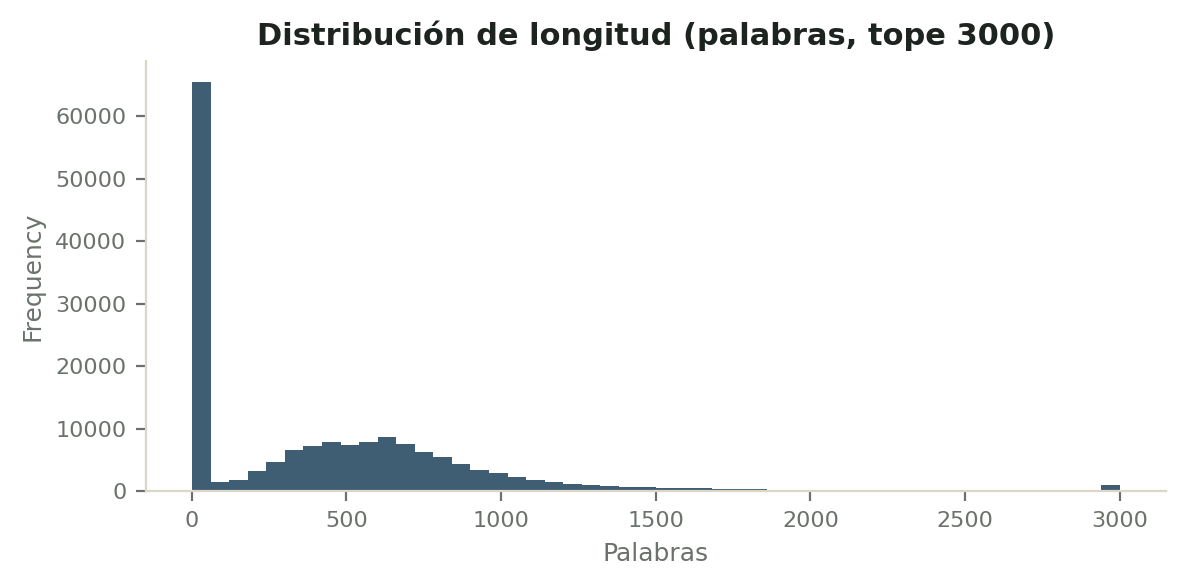
\includegraphics[width=\textwidth]{perfil_longitud.png}
\caption{Distribución de longitud.}
\label{fig:perfil-longitud}
\end{subfigure}

\vspace{0.4cm}
\begin{subfigure}[b]{0.48\textwidth}
\centering
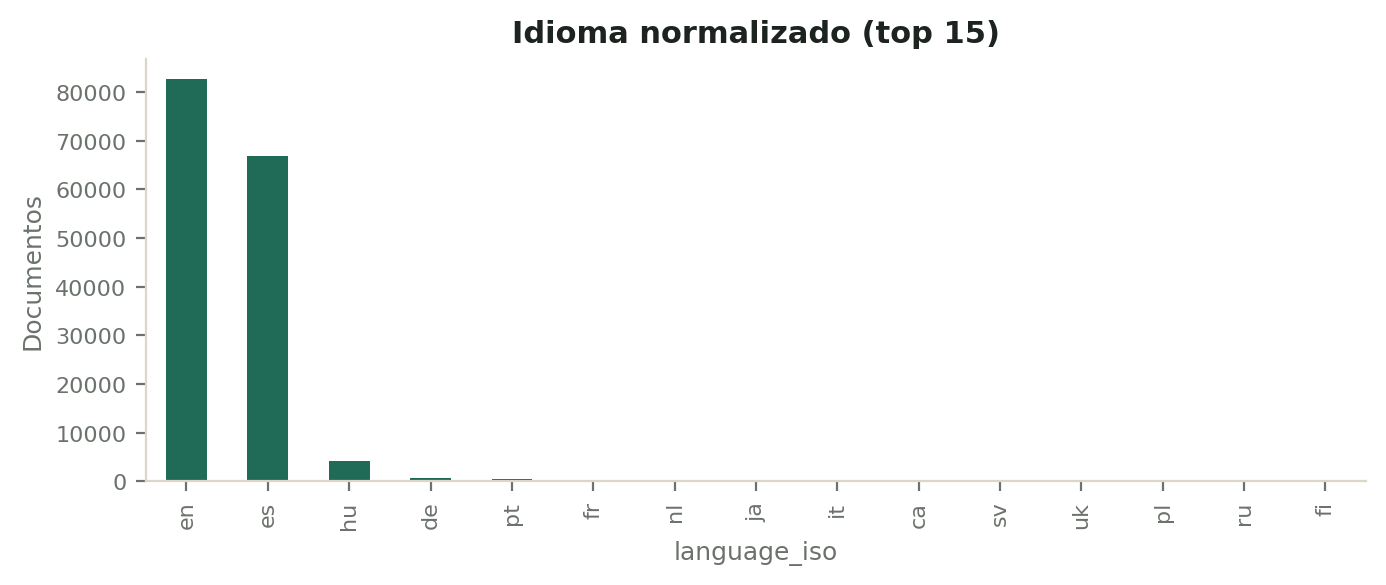
\includegraphics[width=\textwidth]{perfil_idiomas.png}
\caption{Idioma declarado.}
\label{fig:perfil-idiomas}
\end{subfigure}\hfill
\begin{subfigure}[b]{0.48\textwidth}
\centering
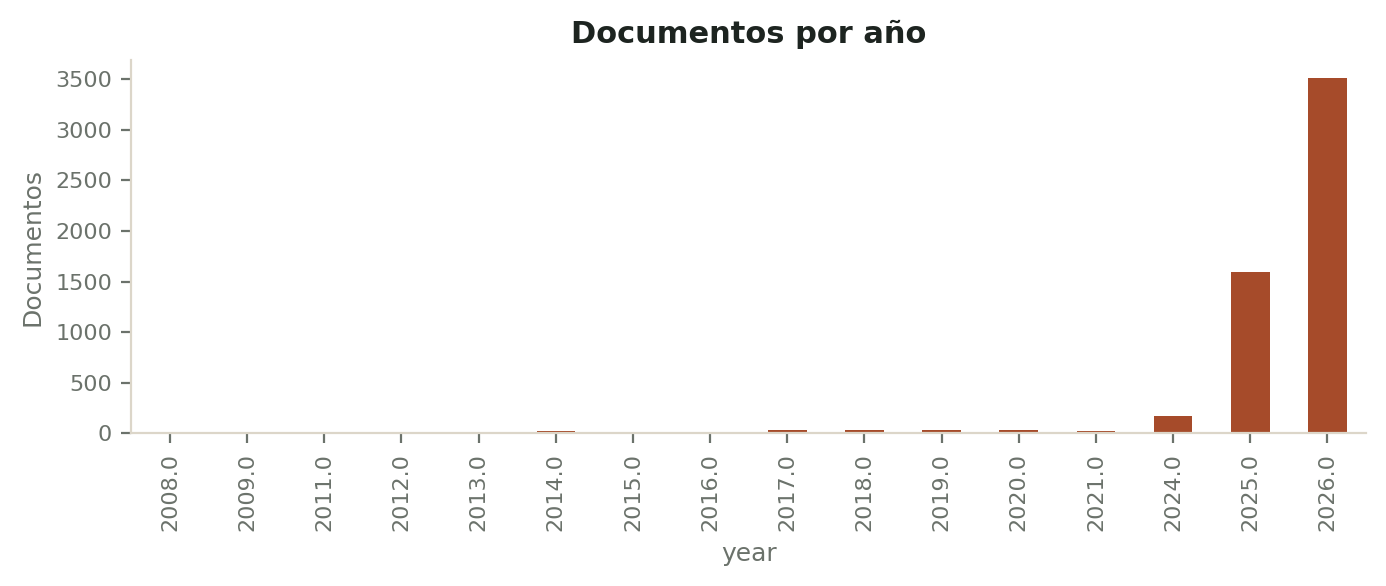
\includegraphics[width=\textwidth]{perfil_anios.png}
\caption{Documentos por año.}
\label{fig:perfil-anios}
\end{subfigure}
\caption{Perfil del corpus: \subref{fig:perfil-colecciones} colecciones, \subref{fig:perfil-longitud} longitud, \subref{fig:perfil-idiomas} idioma y \subref{fig:perfil-anios} distribución temporal.}
\label{fig:perfil}
\end{figure}

\begin{figure}[htbp]
\centering
\begin{subfigure}[b]{0.32\textwidth}
\centering
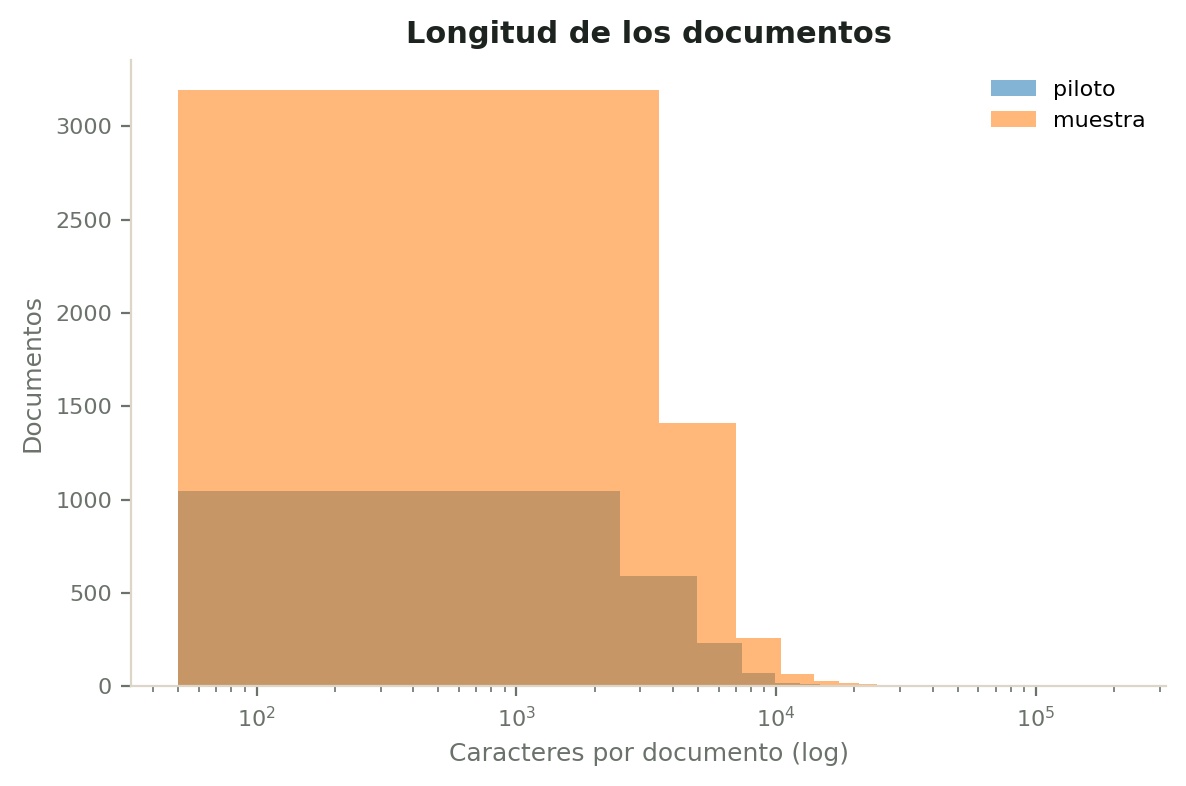
\includegraphics[width=\textwidth]{textometria_longitudes.png}
\caption{Longitudes.}
\label{fig:tex-long}
\end{subfigure}\hfill
\begin{subfigure}[b]{0.32\textwidth}
\centering
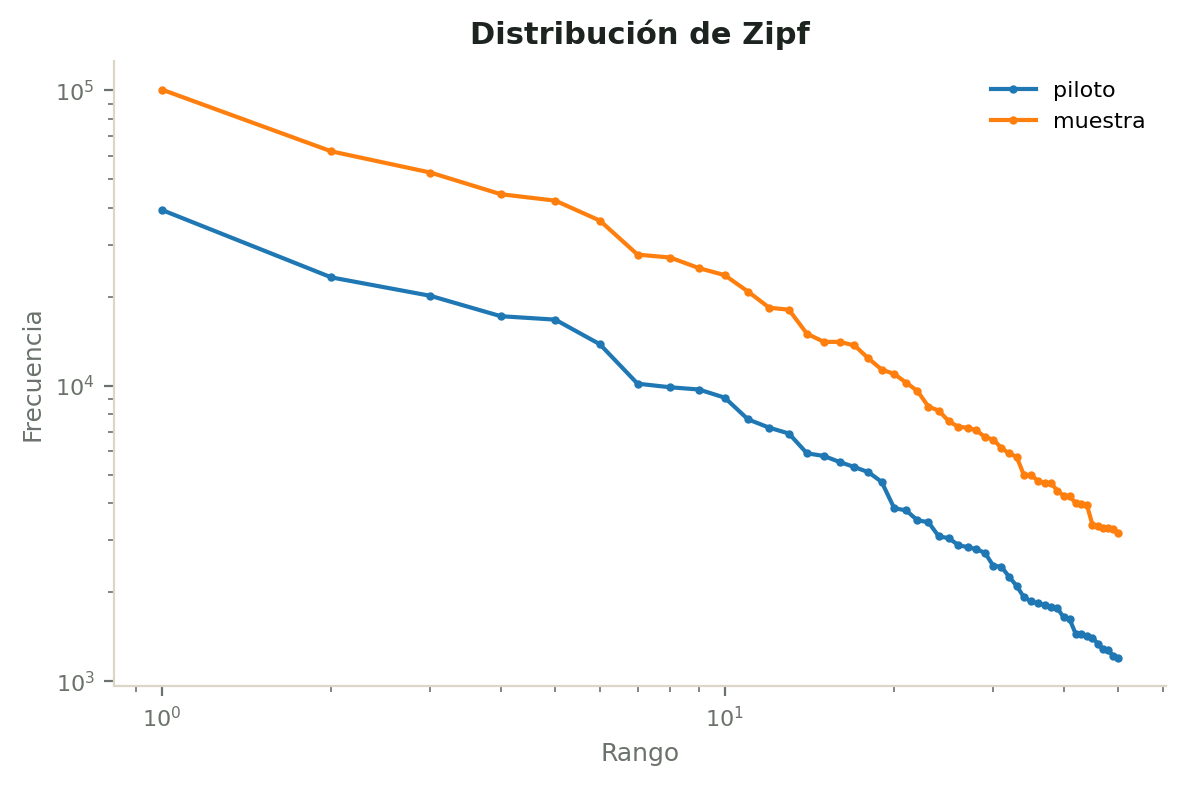
\includegraphics[width=\textwidth]{textometria_zipf.png}
\caption{Zipf.}
\label{fig:tex-zipf}
\end{subfigure}\hfill
\begin{subfigure}[b]{0.32\textwidth}
\centering
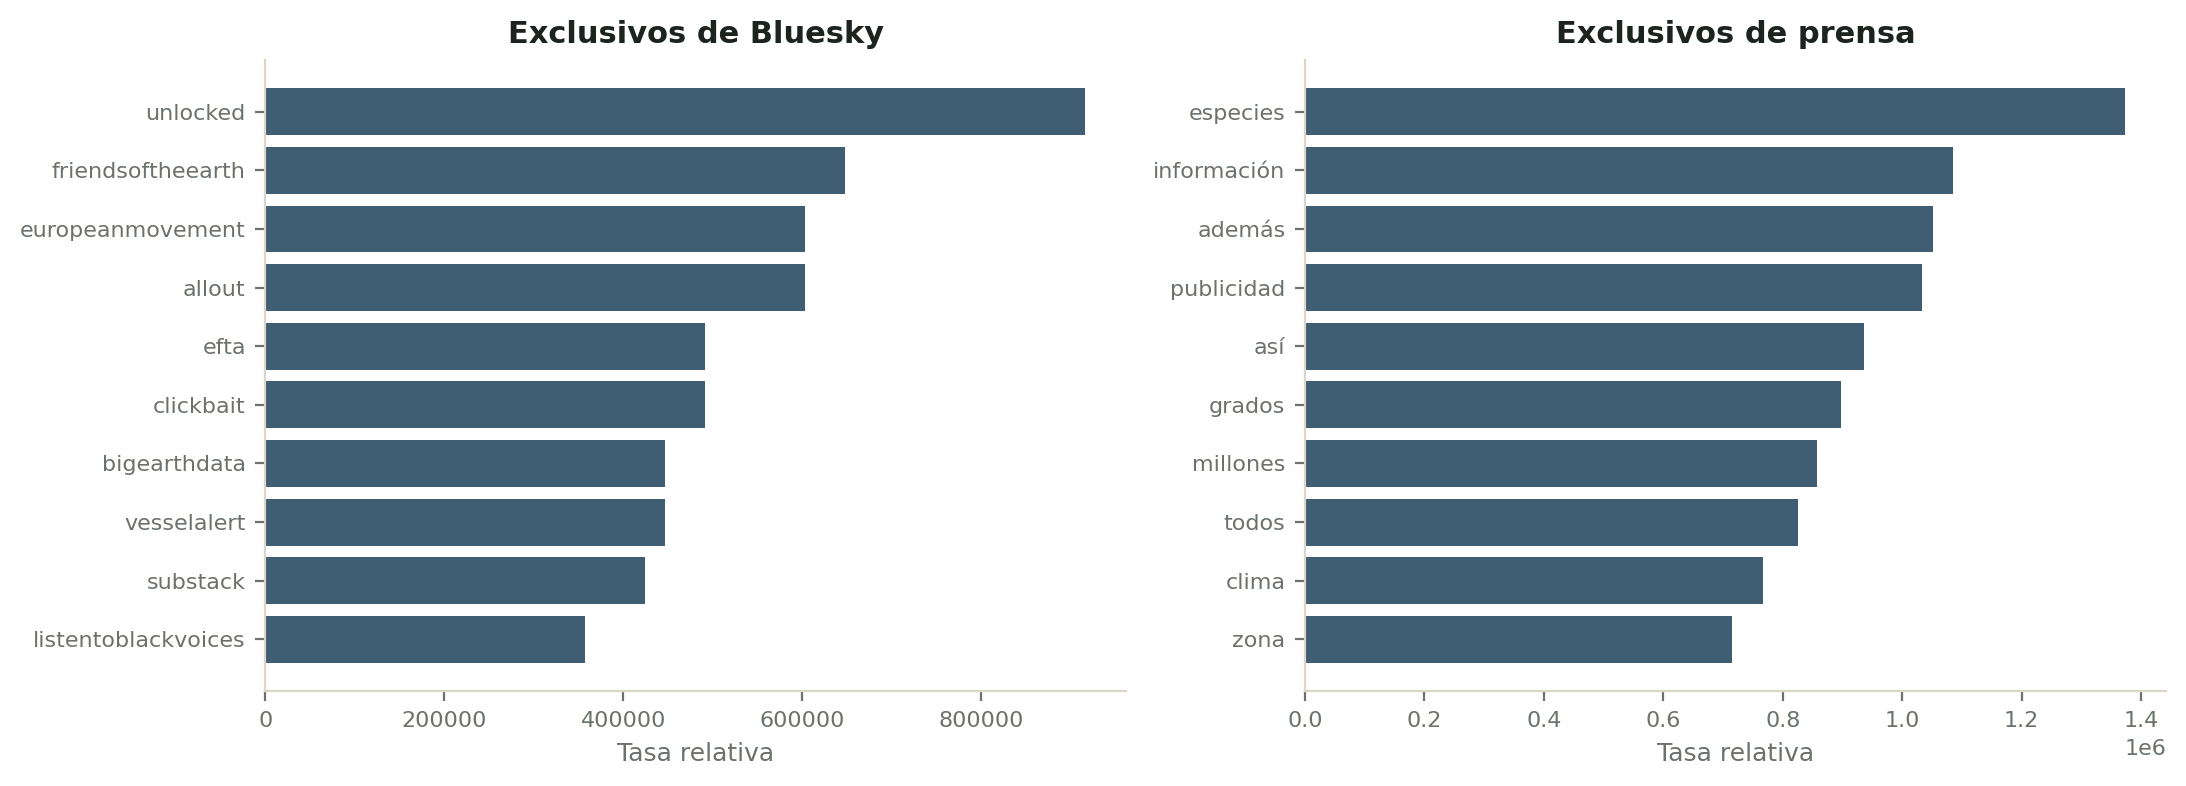
\includegraphics[width=\textwidth]{textometria_terminos.png}
\caption{Términos exclusivos.}
\label{fig:tex-term}
\end{subfigure}

\vspace{0.3cm}
\begin{subfigure}[b]{0.32\textwidth}
\centering
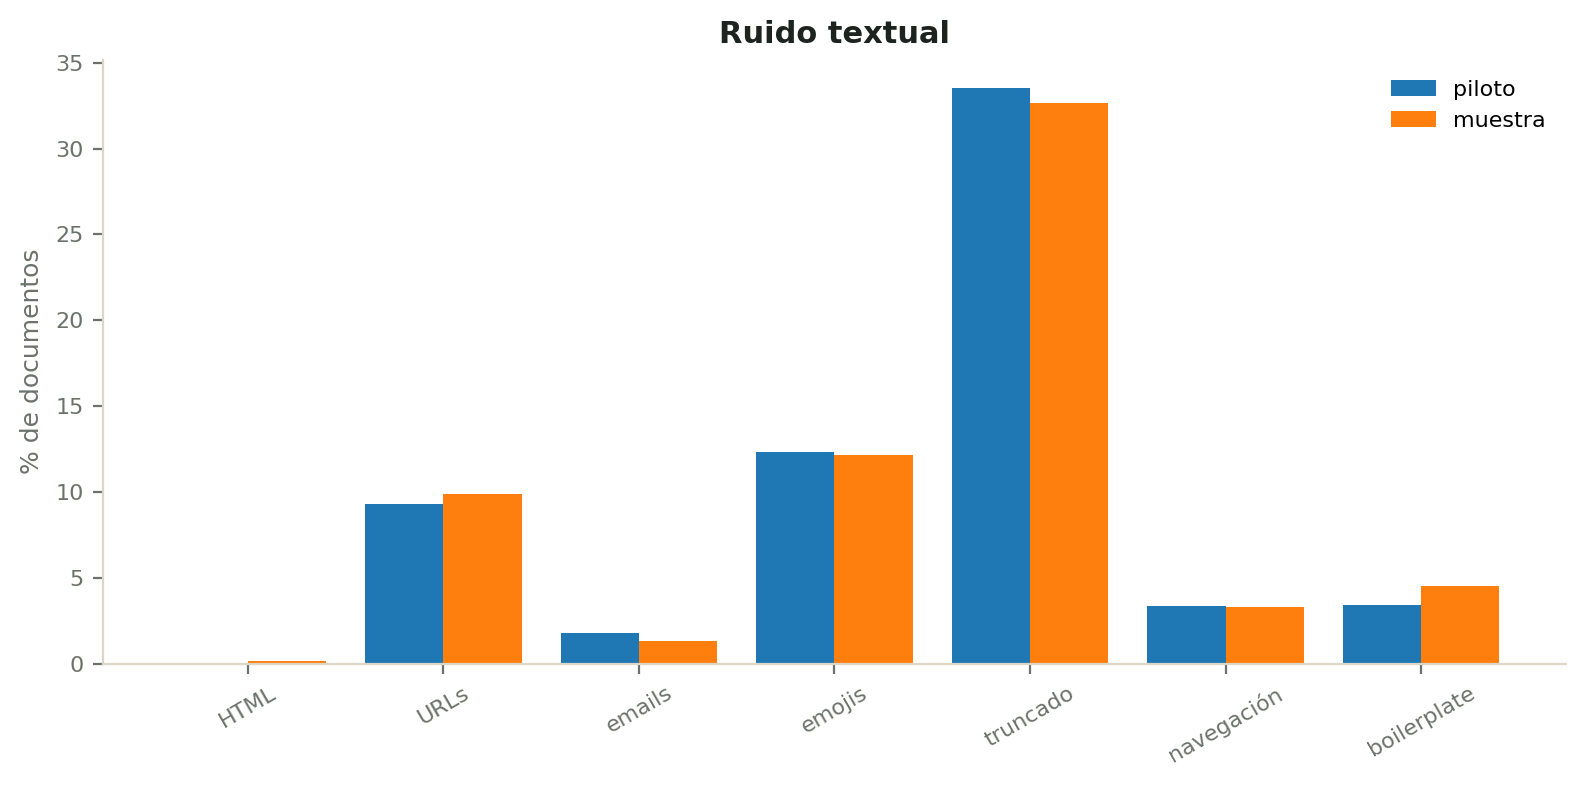
\includegraphics[width=\textwidth]{textometria_ruido.png}
\caption{Ruido.}
\label{fig:tex-ruido}
\end{subfigure}\hfill
\begin{subfigure}[b]{0.32\textwidth}
\centering
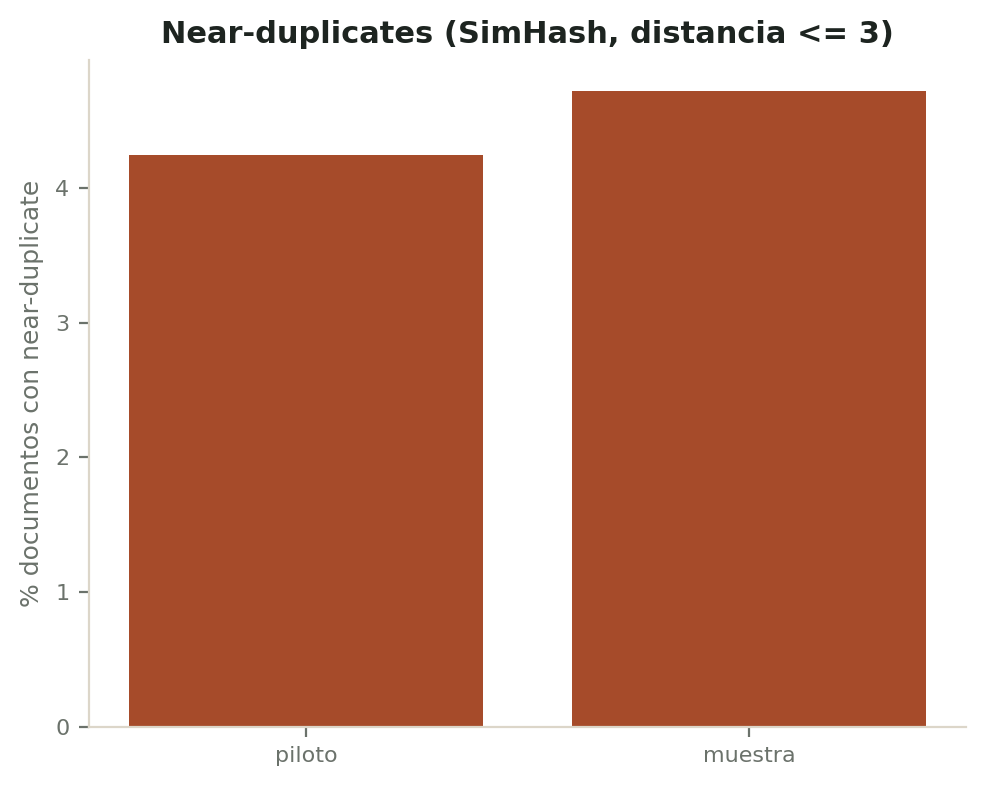
\includegraphics[width=\textwidth]{textometria_near_dups.png}
\caption{Near-duplicates.}
\label{fig:tex-dup}
\end{subfigure}\hfill
\begin{subfigure}[b]{0.32\textwidth}
\centering
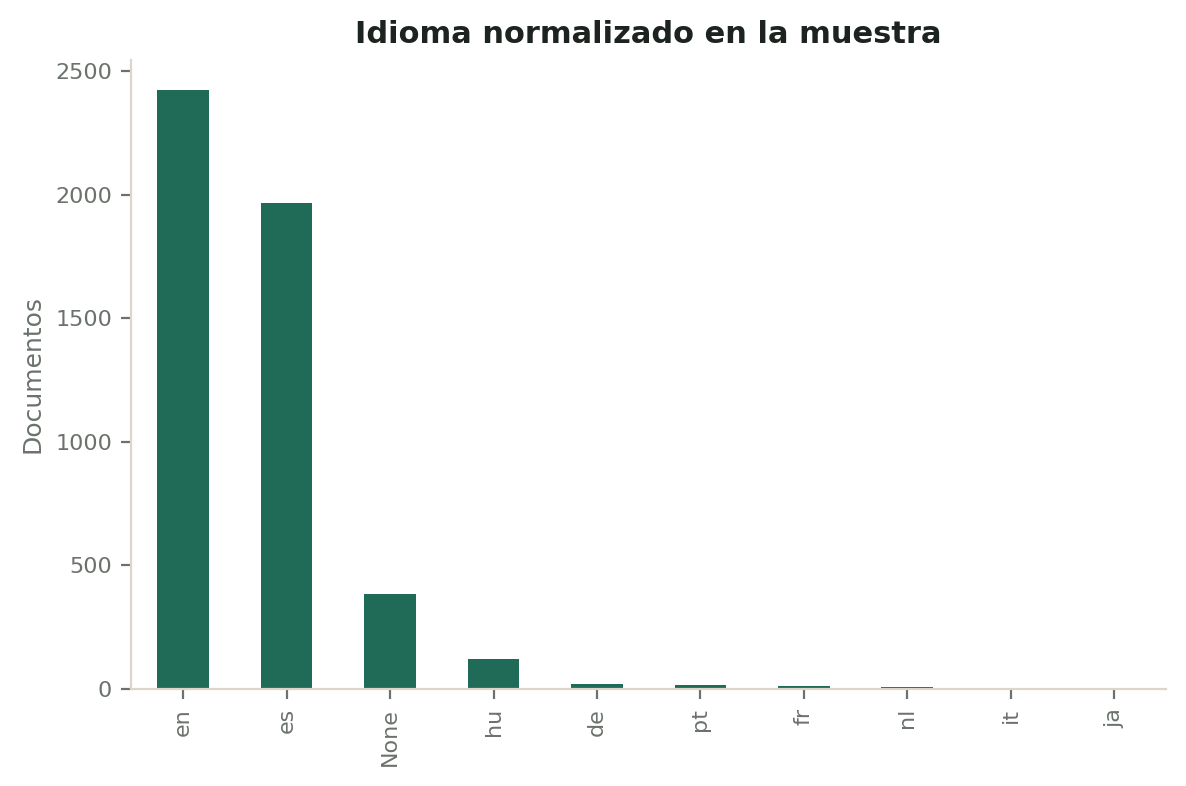
\includegraphics[width=\textwidth]{textometria_idiomas.png}
\caption{Idiomas.}
\label{fig:tex-idio}
\end{subfigure}
\caption{Textometría de la muestra de 5.000 documentos: \subref{fig:tex-long} longitudes, \subref{fig:tex-zipf} ajuste a la ley de Zipf, \subref{fig:tex-term} términos exclusivos por colección, \subref{fig:tex-ruido} ruido, \subref{fig:tex-dup} near-duplicates y \subref{fig:tex-idio} idiomas.}
\label{fig:textometria}
\end{figure}

\section{Arquitectura y decisiones de diseño}

\subsection{Vista general}

El sistema separa la construcción del índice de la consulta. La construcción corre una vez y consume GPU; la consulta corre por pregunta y debe responder en decenas de milisegundos. La Figura~\ref{fig:arquitectura} muestra los dos recorridos y los componentes que los conectan.

\begin{figure}[htbp]
\centering
\shorthandoff{<>}
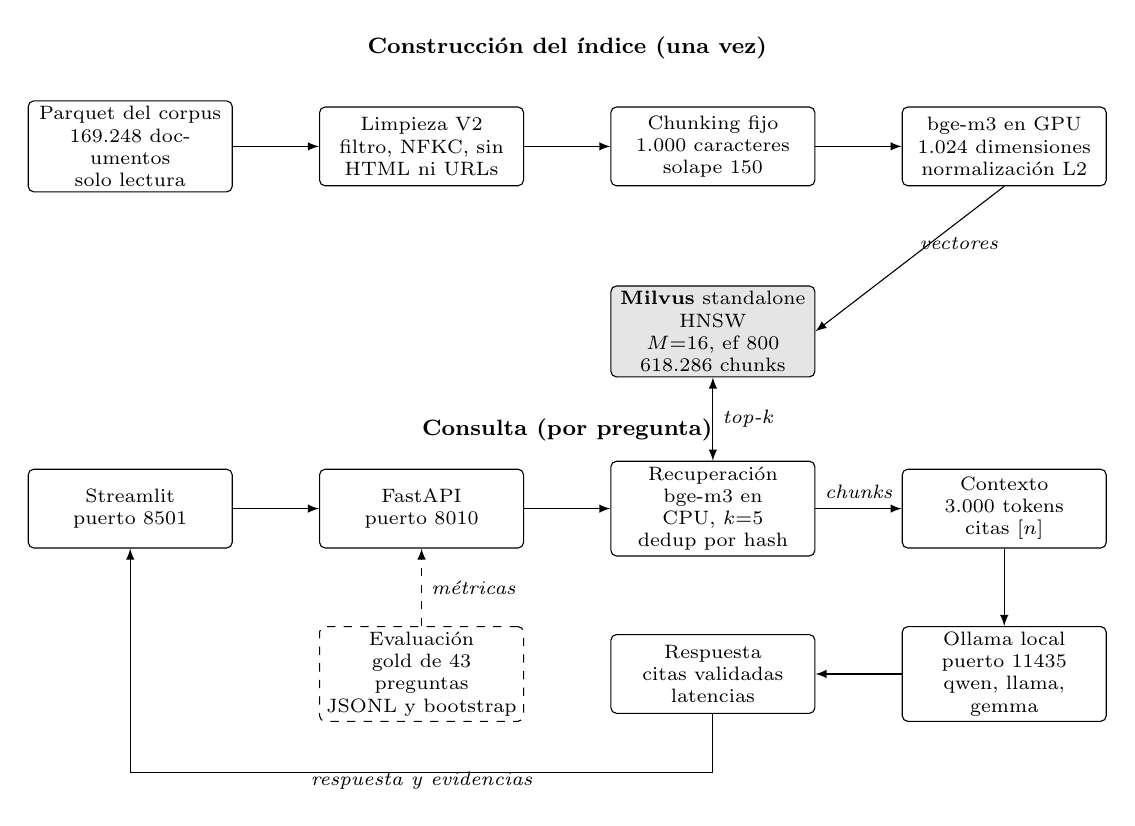
\begin{tikzpicture}[font=\scriptsize, >=latex,
  box/.style={draw, rounded corners=2pt, align=center, text width=2.45cm, minimum height=1.0cm, inner sep=2pt},
  store/.style={box, fill=black!10},
  lbl/.style={font=\scriptsize\itshape, align=center}]

\node[font=\footnotesize\bfseries] at (5.55,1.25) {Construcción del índice (una vez)};

\node[box] (parquet) at (0,0) {Parquet del corpus\\169.248 documentos\\solo lectura};
\node[box] (limpia) at (3.7,0) {Limpieza V2\\filtro, NFKC, sin\\HTML ni URLs};
\node[box] (chunk) at (7.4,0) {Chunking fijo\\1.000 caracteres\\solape 150};
\node[box] (embed) at (11.1,0) {bge-m3 en GPU\\1.024 dimensiones\\normalización L2};

\draw[->] (parquet.east) -- (limpia.west);
\draw[->] (limpia.east) -- (chunk.west);
\draw[->] (chunk.east) -- (embed.west);

\node[store] (milvus) at (7.4,-2.35) {\textbf{Milvus} standalone\\HNSW $M{=}16$, ef 800\\618.286 chunks};

\draw[->] (embed.south) -- (milvus.east) node[lbl, midway, above right] {vectores};

\node[font=\footnotesize\bfseries] at (5.55,-3.6) {Consulta (por pregunta)};

\node[box] (ui) at (0,-4.6) {Streamlit\\puerto 8501};
\node[box] (api) at (3.7,-4.6) {FastAPI\\puerto 8010};
\node[box] (ret) at (7.4,-4.6) {Recuperación\\bge-m3 en CPU, $k{=}5$\\dedup por hash};
\node[box] (ctx) at (11.1,-4.6) {Contexto\\3.000 tokens\\citas $[n]$};

\draw[->] (ui.east) -- (api.west);
\draw[->] (api.east) -- (ret.west);
\draw[<->] (ret.north) -- (milvus.south) node[lbl, midway, right] {top-$k$};
\draw[->] (ret.east) -- (ctx.west) node[lbl, midway, above] {chunks};

\node[box] (ollama) at (11.1,-6.7) {Ollama local\\puerto 11435\\qwen, llama, gemma};
\node[box] (resp) at (7.4,-6.7) {Respuesta\\citas validadas\\latencias};
\node[box, dashed] (eval) at (3.7,-6.7) {Evaluación\\gold de 43 preguntas\\JSONL y bootstrap};

\draw[->] (ctx.south) -- (ollama.north);
\draw[->] (ollama.west) -- (resp.east);
\draw[->, dashed] (eval.north) -- (api.south) node[lbl, midway, right] {métricas};

\draw[->] (resp.south) -- ++(0,-0.75) -| (ui.south);
\node[lbl] at (3.7,-8.05) {respuesta y evidencias};

\end{tikzpicture}
\caption{Arquitectura del sistema. La mitad superior construye el índice; la mitad inferior responde consultas. La evaluación consume la misma API que la interfaz, de modo que las métricas se calculan sobre el camino real de la consulta.}
\label{fig:arquitectura}
\end{figure}

\subsection{Capas y responsabilidades}

La Tabla~\ref{tab:capas} resume los módulos. La separación permitió cambiar el codificador sin tocar la recuperación y comparar cuatro modelos generativos sin volver a indexar.

\begin{table}[htbp]
\centering
\footnotesize
\begin{tabular}{@{}p{2.2cm}p{4.4cm}p{8.4cm}@{}}
\toprule
Capa & Módulo & Responsabilidad \\
\midrule
Ingesta & \texttt{ingest.py} & Lee el Parquet en solo lectura, filtra la muestra y escribe lotes idempotentes. \\
Segmentación & \texttt{chunking.py} & Dos estrategias con offsets sobre el texto original. \\
Embedding & \texttt{embeddings.py} & Un cliente para consultas y pasajes, con prefijos y normalización. \\
Almacenamiento & \texttt{store.py} & Esquema Milvus, índice HNSW, filtros y conteos. \\
Recuperación & \texttt{pipeline.py} & Codifica la consulta, busca, deduplica por hash y mide latencia. \\
Generación & \texttt{pipeline.py} & Arma el contexto por tokens, aplica el prompt y verifica citas. \\
API & \texttt{api.py} & \texttt{/health}, \texttt{/models}, \texttt{/stats}, \texttt{/retrieve}, \texttt{/ask}. \\
Conversación & \texttt{chat.py} & Enrutador, tool calling y guardarraíl de salida con citas válidas. \\
Interfaz & \texttt{ui.py} & Modelo, $k$, filtros, respuesta, evidencias y tiempos. \\
Evaluación & \texttt{evaluate.py}, \texttt{metrics.py} & Corridas crudas y métricas de recuperación y generación. \\
\bottomrule
\end{tabular}
\caption{Capas del sistema y responsabilidad de cada módulo.}
\label{tab:capas}
\end{table}

\subsection{Decisiones que sostienen el diseño}

El registro completo tiene veinte decisiones en formato ADR. La Tabla~\ref{tab:adr} recoge las que explican la forma final del sistema y las consecuencias que se observaron al ejecutarlo.

\begin{table}[htbp]
\centering
\footnotesize
\begin{tabular}{@{}p{0.9cm}p{7.6cm}p{6.2cm}@{}}
\toprule
ADR & Decisión & Consecuencia observada \\
\midrule
001 & Corpus completo con compuerta de rendimiento previa. & La colección final ocupa del orden de 3 a 5 GB. \\
003 & Milvus standalone y una colección por configuración. & Cada cifra de recuperación es atribuible a una sola configuración. \\
004 & Dos estrategias de segmentación, fijo y oraciones. & La comparación cubre una sola dimensión del chunking. \\
006 & Contexto en tokens, citas obligatorias y abstención sin llamar al modelo. & El umbral se calibra en desarrollo y se congela antes de prueba. \\
007 & 20 preguntas de desarrollo y 20 de prueba, 3 repeticiones, 2 anotadores. & El gold final quedó en 43 preguntas, 19 de desarrollo y 24 de prueba. \\
008 & No tocar el origen; deduplicar en la recuperación por hash. & El top-$k$ efectivo puede ser menor que $k$. \\
011 & Piloto de 2.000 documentos primero, corpus completo al final. & La degradación por escala se mide y se reporta como hallazgo. \\
013 & Un compose con dos hosts y perfiles. & El mismo archivo sirve en el equipo local y en el servidor. \\
015 & Red de host porque el demonio no tiene bridge ni iptables. & El compose no es portable a Docker Desktop. \\
016 & e5-base en CPU para el corpus completo; qwen3 queda como comparación. & El umbral de 20 chunks/s solo se cumple con e5 y 24 hilos. \\
018 & Limpieza V2 adoptada por consistencia y costo nulo. & Sin superioridad estadística con 30 preguntas. \\
020 & Ingesta del corpus completo en la GPU local con ROCm. & La imagen pesa del orden de 30 GB. \\
\bottomrule
\end{tabular}
\caption{Decisiones de arquitectura con mayor efecto sobre los resultados.}
\label{tab:adr}
\end{table}

ADR-016 se revisó en E10: el corpus completo se reindexó con bge-m3 en fp16 sobre la RX 9070 y e5-base quedó como referencia de las ablaciones. El gold de ADR-019 se amplió en E12 con 17 documentos de consenso, sin cambiar las 43 preguntas.

\clearpage
\subsection{Despliegue}

Todos los servicios usan red de host porque el demonio de Docker del equipo tiene \texttt{iptables:~false} y \texttt{bridge:~none}. Los puertos son Milvus 19530 y 9091, MinIO 9000 y 9001, Ollama 11435, API 8010 y Streamlit 8501. El Ollama nativo del equipo se queda en 11434 y sirve de respaldo.

La ingesta del corpus completo corre en un contenedor construido sobre la imagen de ROCm 7.2.4, con acceso a \texttt{/dev/kfd} y \texttt{/dev/dri}. La medición de rendimiento justifica la decisión: e5-base procesa 25,5 chunks por segundo en CPU con 24 hilos y 106,9 en la RX 9070 XT con lote de 128. La diferencia convierte una ingesta de 11 a 12 horas en una de 2 a 3 horas. La API sigue consultando en CPU con el mismo modelo; las diferencias de coma flotante entre dispositivos son despreciables y no cambian el vecindario recuperado de forma medible.

\section{Método}

\subsection{Limpieza}

Se compararon cuatro variantes acumulativas. V0 es el texto crudo. V1 descarta las páginas de error del crawler. V2 añade normalización NFKC, elimina HTML y URLs y colapsa espacios. V3 añade deduplicación de near-duplicates por chunk. La limpieza se aplica al texto de cada chunk en el momento de indexar; \texttt{position} y \texttt{end\_offset} siguen referidos al texto original, de modo que la trazabilidad no se pierde. El hash del chunk se calcula sobre el texto limpio.

\subsection{Segmentación}

La estrategia adoptada es el chunking fijo de 1.000 caracteres con 150 de solape. Los identificadores son deterministas y se derivan del documento, la estrategia, el tamaño, el solape y el offset, lo que hace la ingesta idempotente. La alternativa comparada corta por oraciones con un máximo de 384 tokens y solape de una oración, con corte duro solo cuando una oración excede el límite.

\subsection{Codificación}

\begin{sloppypar}
Los tres codificadores comparados son bi-encoders que se consultan por similitud coseno \cite{reimers2019sbert}. El que sostiene las ablaciones de limpieza, segmentación y $k$ es \path{intfloat/multilingual-e5-base}, con vectores de 768 dimensiones, prefijos \texttt{query:} y \texttt{passage:} según el uso previsto del modelo \cite{wang2024e5} y normalización L2 para que la similitud coseno sea un producto interno; se usa a través de \texttt{sentence-transformers} \cite{sbertdocs}.

El codificador del sistema final es \path{BAAI/bge-m3}, de 1.024 dimensiones \cite{chen2024bge}, adoptado en E10 tras medirlo sobre el corpus completo. El tercer codificador es \path{qwen3-embedding:8b}, servido por Ollama, con vectores de 4.096 dimensiones truncados a 1.024 por representación multinivel y renormalizados; las consultas llevan el prefijo \path{Instruct: ...\nQuery: ...} y los documentos van sin prefijo.
\end{sloppypar}

\subsection{Índice y recuperación}

Milvus standalone con etcd y MinIO como infraestructura. El índice es HNSW con $M=16$ y 200 candidatos en la construcción, y la métrica es COSINE \cite{malkov2020hnsw,milvusdocs}. Las ablaciones exploraron 200 vecinos y el sistema final usa \texttt{ef}=800 (Sección~\ref{sec:ajuste}). El valor de \texttt{ef} afecta el recall: con \texttt{ef}=64 el recall@10 del conjunto de humo era 0,880 y con 200 subió a 0,960. Cada configuración de chunking y codificador tiene su propia colección, y cambiar cualquiera de las dos exige una colección nueva. Los filtros por idioma y fecha se aplican como expresiones escalares dentro de la búsqueda.

\subsection{Generación, citas y abstención}

El contexto se mide en tokens estimados y se corta antes de llamar al modelo, con un presupuesto por defecto de 3.000. El prompt delimita la evidencia, numera los fragmentos y exige citas en la forma \texttt{[n]}. Después de generar, el sistema valida que cada índice citado exista en el contexto y registra \texttt{invalid\_citations}. La abstención ocurre sin llamar al modelo cuando no hay evidencia recuperada o cuando la mejor puntuación no supera el umbral calibrado en desarrollo. La decisión se apoya en que los modelos de 1 a 3 mil millones de parámetros no son fiables para decidir por sí mismos cuándo callar.

Los cuatro modelos se sirven con Ollama \cite{ollamadocs}. La ruta conversacional añade un enrutador que decide si la consulta requiere el corpus y un guardarraíl de salida: un modelo juez, \texttt{llama3.2:3b} por defecto, decide si la evidencia contiene la respuesta, y el sistema se abstiene cuando el juez responde que no. Los saludos y la charla no pasan por el corpus. Esa ruta no se evalúa en este informe: las métricas de E4 se calcularon sobre el camino directo de \texttt{/ask}.

\subsection{API e interfaz}

FastAPI expone \texttt{/health}, \texttt{/models}, \texttt{/stats}, \texttt{/retrieve} y \texttt{/ask} \cite{fastapidocs}. La respuesta de \texttt{/ask} incluye la respuesta, la evidencia, las latencias por etapa, los tokens por segundo, la versión y el hash del prompt, las citas y las citas inválidas. Streamlit consume esa API y permite elegir modelo, $k$, idioma, rango de fechas y colección \cite{streamlitdocs}. La interfaz muestra las fuentes con enlace y los tiempos por etapa, porque en la demostración la latencia es tan visible como la respuesta.

\section{Protocolo de evaluación}

\subsection{Compuerta de humo}

Antes de escalar se ejecutó una compuerta sobre 600 documentos (582 tras el filtro de calidad), 53 preguntas generadas desde los documentos, 3 repeticiones y $k=10$. La compuerta exigía Recall@10 de documento igual a 1,00, MRR@10 de 0,85, nDCG@10 de 0,85, cobertura de span en el top-5 de 0,90, cero duplicados, cero offsets rotos, top-10 determinista en tres corridas y filtros exactos. La Tabla~\ref{tab:humo} muestra la evolución.

\begin{table}[htbp]
\centering
\footnotesize
\begin{tabular}{@{}llrrrrr@{}}
\toprule
Versión & Cambio & Preguntas & Recall@10 & MRR@10 & nDCG@10 & Span top-10 \\
\midrule
v1 & índice con ruido, ef=64 & 53 & 0,849 & 0,811 & 0,821 & 0,830 \\
v2 & sin documentos de error, ef=64 & 53 & 0,943 & 0,877 & 0,894 & 0,906 \\
v3 & 3 preguntas excluidas, ef=64 & 50 & 0,880 & 0,840 & 0,850 & 0,840 \\
final & 15 preguntas excluidas, ef=200 & 38 & \textbf{1,000} & \textbf{0,987} & \textbf{0,990} & \textbf{0,947} \\
\bottomrule
\end{tabular}
\caption{Compuerta de humo sobre 600 documentos y 3 repeticiones.}
\label{tab:humo}
\end{table}

El diagnóstico de la compuerta produjo tres correcciones que se conservaron en el sistema final. La primera fue el filtro de calidad: las páginas de error del crawler dominaban el top-10 de cualquier consulta. La segunda fue subir \texttt{ef} de 64 a 200; la ablación sobre las 50 preguntas dio 0,880 con 64, 0,920 con 128, 0,960 con 200 y 0,960 con 400, así que 200 es el punto donde la curva se aplana. La tercera fue excluir 15 preguntas por criterio explícito: tasas de cambio respondidas por varios documentos, referencias vagas (``el país'', ``la medida'', ``la empresa AG''), una pregunta en ruso sobre un documento en ucraniano y una generada desde el boilerplate del portal. La lista y la razón de cada exclusión están en el archivo del gold de humo.

La conclusión de la compuerta es acotada: el pipeline recupera correctamente en un conjunto pequeño y curado. No es una prueba de calidad a escala, y el resto del informe se encarga de mostrar por qué.

\subsection{Gold de evaluación}

El gold consolidado tiene 43 preguntas: 19 de desarrollo y 24 de prueba. De las 43, 38 son respondibles y 5 no tienen respuesta en el corpus. Las 38 respondibles son directas: 36 vienen de prensa y 2 de Bluesky. Por idioma, 34 están en español y 9 en inglés. Carlos revisó las 43 filas, marcó 31 con ``Sí'' y 12 con ``Corregir''; las 12 correcciones se aplicaron y cada una quedó con una nota de revisión. Julián revisó 40 de las 43 en una segunda pasada: 30 confirmadas, 8 corregidas y 2 rechazadas sin cambio; Erika y Óscar no revisaron. Tres preguntas no se pudieron verificar por enlaces caídos.

Sobre la colección del piloto con limpieza V2, $k=10$ y 3 repeticiones, el gold da Recall@10 de 0,947 con IC [0,904; 0,983], P@1 de 0,842, P@5 de 0,947, MRR@10 de 0,895, nDCG@10 de 0,909 con IC [0,862; 0,950] y cobertura de span de 0,895. Los dos fallos son las preguntas g-045 y g-046. En ambos casos el documento está en la colección: son fallos de recuperación, no referencias rotas.

\subsection{Métricas}

Se reportan Recall@$k$, Precision@1 y @5, MRR@10, MAP@10, nDCG@10, cobertura de span, citas válidas, abstención, latencia por etapa y tokens por segundo. La evaluación de RAG admite además métricas de utilidad downstream y jueces automáticos \cite{salemi2024erag,es2023ragas,saadfalcon2024ares,ru2024ragchecker}; aquí se usan solo como complemento de la anotación humana y no como veredicto. La precisión@$k$ no se usa para decidir: con un solo documento relevante por pregunta está acotada por $1/k$ (0,10 con $k=10$) y su valor depende del número de documentos devueltos. Por eso las decisiones se toman con Recall, P@1, P@5, MRR y nDCG. La cobertura de span se reporta como métrica secundaria en las variantes limpias, porque el span anotado viene del texto crudo y la limpieza modifica el texto indexado.

\subsection{Estadística}

La unidad de remuestreo es la pregunta, no la repetición. Los intervalos se calculan con bootstrap percentil de 1.000 remuestreos. Dos configuraciones se comparan con bootstrap pareado sobre las mismas preguntas: si el intervalo de la diferencia contiene cero, no se declara superioridad. En las comparaciones múltiples se aplica Bonferroni. En la ablación de limpieza se prueban 7 métricas por 3 variantes, 21 pruebas, y el nivel de cada intervalo se ajusta a $0,05/21$. En E1 se prueban 7 métricas y el ajuste es $0,05/7$. Con 20 o 30 preguntas se reporta el intervalo, no solo la media, y un resultado perfecto se interpreta como compuerta de correctitud, no como prueba de calidad.

\section{Experimentos y resultados}

\subsection{Limpieza: V0 a V3}
\label{sec:limpieza}

El experimento se hizo sobre el piloto de 2.000 documentos, con 30 preguntas (25 de prensa y 5 de Bluesky), 3 repeticiones, $k=10$, e5-base, el mismo chunking y el mismo índice. Cada variante tiene su colección. El gold de humo no se usó porque su muestra de 600 documentos no es subconjunto del piloto: sus referencias no existen en estas colecciones. Esa separación se detectó al medir y quedó como lección de diseño.

La Tabla~\ref{tab:limpieza} presenta las métricas y la Figura~\ref{fig:limpieza} las compara visualmente.

\begin{table}[htbp]
\centering
\footnotesize
\begin{tabular}{@{}lrrrrrr@{}}
\toprule
Variante & P@1 & P@5 & Recall@10 & IC 95\,\% recall & MRR@10 & nDCG@10 \\
\midrule
V0 crudo & 0,733 & 0,833 & 0,833 & [0,700; 0,967] & 0,775 & 0,790 \\
V1 filtro de ruido & 0,767 & 0,833 & 0,833 & [0,700; 0,967] & 0,800 & 0,809 \\
V2 normalización conservadora & \textbf{0,833} & \textbf{0,900} & \textbf{0,900} & [0,767; 1,000] & \textbf{0,867} & \textbf{0,875} \\
V3 V2 + dedup de chunks & 0,800 & 0,867 & 0,867 & [0,733; 0,967] & 0,833 & 0,842 \\
\bottomrule
\end{tabular}
\caption{Ablación de limpieza sobre 30 preguntas del piloto, $k=10$, 3 repeticiones.}
\label{tab:limpieza}
\end{table}

\begin{figure}[htbp]
\centering
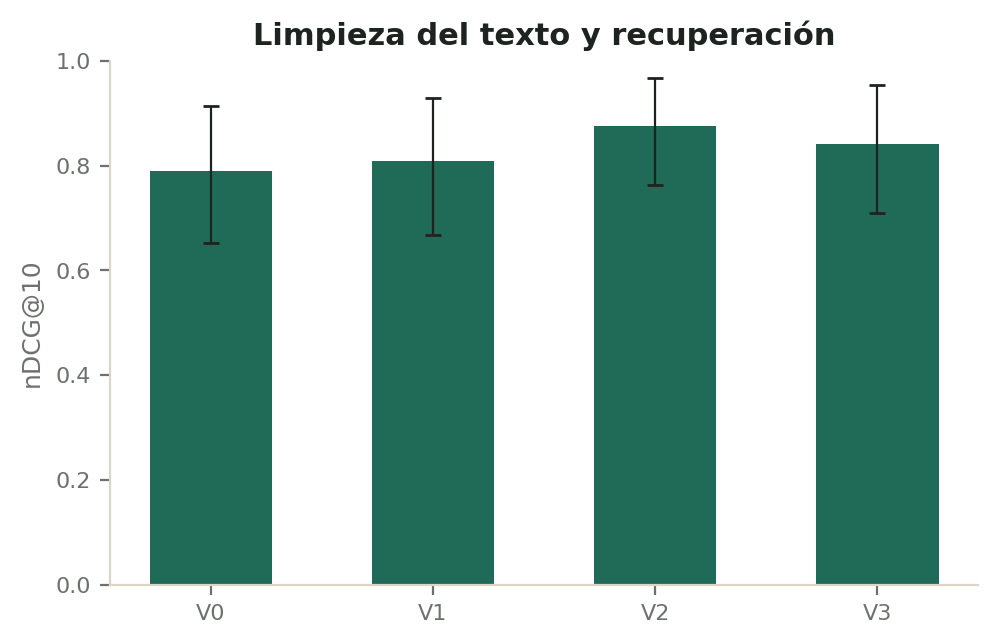
\includegraphics[width=0.82\textwidth]{limpieza_comparacion.png}
\caption{Métricas de recuperación por variante de limpieza sobre las 30 preguntas del piloto.}
\label{fig:limpieza}
\end{figure}

V2 tiene la mejor estimación puntual en las cuatro métricas de calidad, con una ganancia de 10 puntos de P@1, 6,7 de P@5 y Recall@10, y 8,6 de nDCG@10 frente al texto crudo. La Tabla~\ref{tab:bonferroni} muestra por qué esa ganancia no se declara significativa.

\begin{table}[htbp]
\centering
\footnotesize
\begin{tabular}{@{}llrrr@{}}
\toprule
Variante & Métrica & Diferencia & IC ajustado & ¿Excluye cero? \\
\midrule
V1 & P@1 & $+0,033$ & $[-0,160;\,0,200]$ & No \\
V1 & Recall@10 & $0,000$ & $[-0,100;\,0,160]$ & No \\
V1 & nDCG@10 & $+0,019$ & $[-0,133;\,0,143]$ & No \\
V2 & P@1 & $+0,100$ & $[0,000;\,0,267]$ & No (toca cero) \\
V2 & P@5 & $+0,067$ & $[0,000;\,0,200]$ & No (toca cero) \\
V2 & Recall@10 & $+0,067$ & $[0,000;\,0,233]$ & No (toca cero) \\
V2 & nDCG@10 & $+0,086$ & $[0,000;\,0,252]$ & No (toca cero) \\
V3 & P@1 & $+0,067$ & $[-0,133;\,0,260]$ & No \\
V3 & nDCG@10 & $+0,052$ & $[-0,133;\,0,228]$ & No \\
\bottomrule
\end{tabular}
\caption{Bootstrap pareado contra V0 con corrección de Bonferroni sobre 21 pruebas.}
\label{tab:bonferroni}
\end{table}

Ninguna comparación de calidad excluye cero. V2 toca el límite inferior en cuatro métricas, lo que es compatible con una mejora real pequeña y con ausencia de efecto. La decisión de adoptar V2 se sostiene en tres razones que no son estadísticas: la consistencia de la estimación en todas las métricas, el costo nulo (la limpieza no añade tiempo de consulta) y el hecho de que elimina 68 páginas de error que de otro modo entrarían al índice.

El desglose ayuda a entender dónde se concentra la ganancia. En prensa (25 preguntas) el nDCG pasa de 0,908 en V0 a 0,971 en V2; en inglés (9 preguntas) de 0,381 a 0,667. En español (21 preguntas) no cambia, porque V0 ya estaba en 0,965. En Bluesky (5 preguntas) las cuatro variantes quedan entre 0,200 y 0,400, con tres preguntas vagas que explican el nivel y un tamaño de muestra que no permite concluir.

\subsection{E1: segmentación por oraciones contra chunking fijo}

El experimento usó las mismas 30 preguntas, 3 repeticiones, e5-base, limpieza V2 y \texttt{ef=200}. La Tabla~\ref{tab:e1} y la Figura~\ref{fig:e1} resumen el resultado.

\begin{table}[htbp]
\centering
\footnotesize
\begin{tabular}{@{}lrrrrrrr@{}}
\toprule
Variante & Chunks & P@1 & P@5 & Recall@10 & MRR@10 & nDCG@10 & p50 \\
\midrule
Fijo 1000/150 & 7.280 & \textbf{0,833} & \textbf{0,900} & \textbf{0,900} & \textbf{0,867} & \textbf{0,875} & \textbf{38,5 ms} \\
Oraciones 384/1 & 5.163 & 0,767 & 0,833 & 0,833 & 0,794 & 0,804 & 42,1 ms \\
\bottomrule
\end{tabular}
\caption{E1: chunking fijo contra segmentación por oraciones, 30 preguntas.}
\label{tab:e1}
\end{table}

\begin{figure}[htbp]
\centering
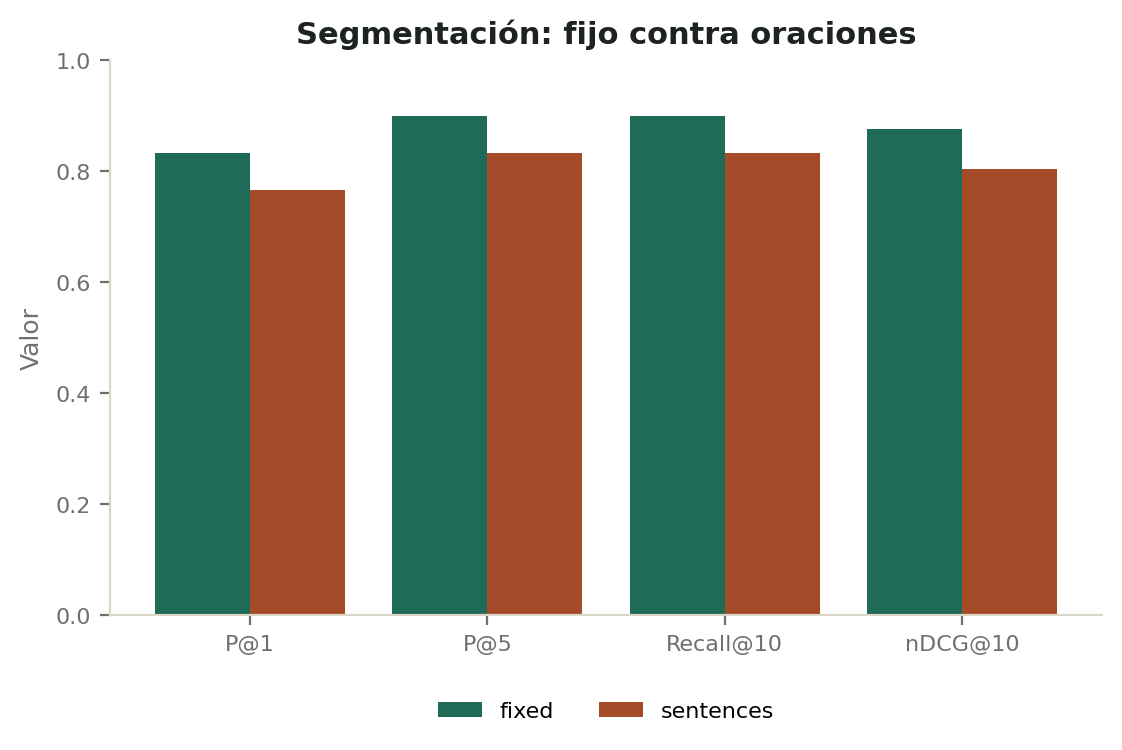
\includegraphics[width=0.78\textwidth]{e1_chunking.png}
\caption{Comparación de las dos estrategias de segmentación sobre las 30 preguntas del piloto.}
\label{fig:e1}
\end{figure}

El bootstrap pareado con Bonferroni sobre 7 pruebas da, para oraciones menos fijo, nDCG de $-0,071$ con IC $[-0,221;\,0,025]$, recall de $-0,067$ con IC $[-0,233;\,0,000]$ y P@1 de $-0,067$ con IC $[-0,233;\,0,114]$. Ninguna diferencia de calidad excluye cero. La latencia sí lo hace: el fijo es 3,65 ms más rápido, con IC $[2,25;\,4,97]$. La decisión es mantener el fijo: mejor estimación puntual en las seis métricas, más rápido y con más chunks, lo que da más granularidad al contexto. Las oraciones no aportan con este gold, aunque tampoco se puede afirmar que sean peores.

\subsection{E2: tamaño del contexto recuperado}

Se compararon $k=3$, $k=5$ y $k=10$ sobre la mejor colección, con las mismas 30 preguntas y 3 repeticiones. La Tabla~\ref{tab:e2} muestra el resultado.

\begin{table}[htbp]
\centering
\footnotesize
\begin{tabular}{@{}lrrrrrr@{}}
\toprule
$k$ & P@1 & P@5 & Recall@$k$ & MRR@$k$ & nDCG@$k$ & Recuperación p50 \\
\midrule
3 & 0,833 & 0,900 & 0,900 & 0,867 & 0,875 & 40,1 ms \\
5 & 0,833 & 0,900 & 0,900 & 0,867 & 0,875 & 39,4 ms \\
10 & 0,833 & 0,900 & 0,900 & 0,867 & 0,875 & 38,5 ms \\
\bottomrule
\end{tabular}
\caption{E2: ablación del tamaño de contexto, 30 preguntas.}
\label{tab:e2}
\end{table}

\begin{figure}[htbp]
\centering
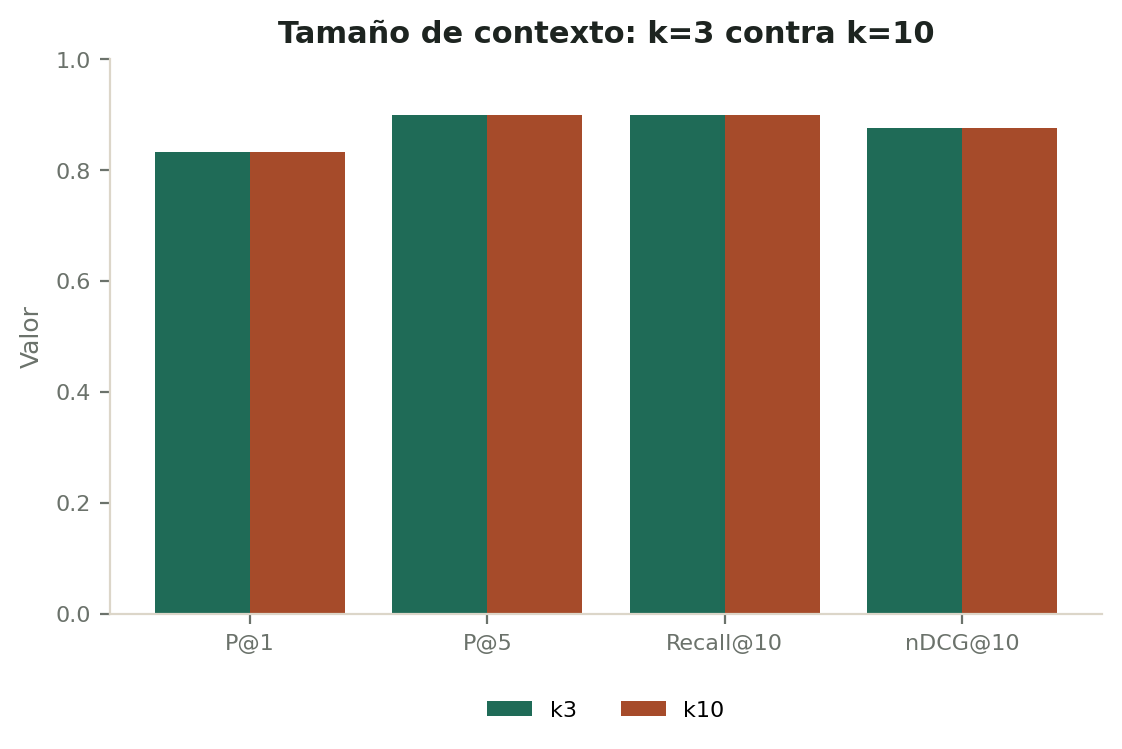
\includegraphics[width=0.78\textwidth]{e2_k3_vs_k10.png}
\caption{Métricas de recuperación para $k=3$ y $k=10$; los valores son idénticos.}
\label{fig:e2}
\end{figure}

Las tres configuraciones devuelven exactamente las mismas métricas de calidad: el documento relevante está siempre en el top 3. La única diferencia significativa es la latencia, y va en la dirección esperada: $k=3$ tarda 1,64 ms menos que $k=10$ con IC $[-2,85;\,-0,57]$, y $k=5$ tarda 0,94 ms menos con IC $[-1,76;\,-0,15]$. Son milisegundos, no un cambio de calidad. Se fija $k=5$ como margen para preguntas comparativas que no están en este conjunto, sabiendo que con el gold actual no hay ganancia medible de 3 a 5 ni de 5 a 10. El costo de $k=5$ es más contexto en generación, no más latencia de recuperación.

\subsection{E3: codificador}

Se compararon e5-base y qwen3-embedding:8b sobre el piloto, con 18 preguntas de desarrollo, 3 repeticiones, $k=10$, mismas preguntas y el mismo índice limpio. La Tabla~\ref{tab:e3} presenta calidad y latencia.

\begin{table}[htbp]
\centering
\footnotesize
\begin{tabular}{@{}lrrrrrr@{}}
\toprule
Codificador & Hit@10 & Recall@10 & MRR@10 & nDCG@10 & Span top-10 & p50 \\
\midrule
e5-base 768 & 0,944 & 0,944 & 0,757 & 0,802 & 0,944 & \textbf{37 ms} \\
qwen3-embedding:8b 1024 & \textbf{1,000} & \textbf{1,000} & \textbf{0,821} & \textbf{0,866} & 0,944 & 68 ms \\
\bottomrule
\end{tabular}
\caption{E3: comparación de codificadores sobre el piloto, 18 preguntas de desarrollo.}
\label{tab:e3}
\end{table}

qwen recupera mejor en el piloto: Recall@10 perfecto y 6,4 puntos más de nDCG@10. El problema es el costo. Medido con lotes de 16 textos de unos 900 caracteres, qwen3-embedding:8b rinde 1,9 chunks por segundo en la GTX 1080 del servidor y 7,3 en la RX 9070 XT local. Para 618.286 chunks, el servidor tardaría 88 horas y la GPU local 23. e5-base rinde 12,2 con 8 hilos y 25,5 con 24 hilos, y la ingesta en GPU llega a 106,9. La decisión es adoptar e5-base para producción y conservar qwen como comparación documentada (ADR-016). No es una preferencia de calidad: es la única opción que cabe en el presupuesto de tiempo del taller.

\subsection{E4: modelos generativos}

El diseño compara cuatro modelos con la misma evidencia: 24 preguntas de prueba (19 respondibles y 5 sin respuesta), 3 repeticiones, temperatura 0, $k=5$ y la colección del piloto con limpieza V2. La recuperación es idéntica entre modelos, con hit@5 de 0,947, P@1 de 0,737, P@5 de 0,947, MRR de 0,842, nDCG@5 de 0,870 y cobertura de span de 0,947. Cualquier diferencia en la respuesta es atribuible al modelo y no al recuperador.

\begin{table}[htbp]
\centering
\footnotesize
\begin{tabular}{@{}lrrrrrr@{}}
\toprule
Modelo & Generación p50 & Tokens/s & Abstención & Sin citas & Citas inválidas & Abstención en sin respuesta \\
\midrule
gemma2:2b & 323 ms & 181 & 5,3\,\% & \textbf{0,0\,\%} & 0 & 12/15 \\
qwen2.5:1.5b & \textbf{212 ms} & 261 & 10,5\,\% & 89,5\,\% & 0 & \textbf{15/15} \\
llama3.2:3b & 285 ms & 182 & 15,8\,\% & 56,1\,\% & 0 & \textbf{15/15} \\
llama3.2:1b & 84 ms & \textbf{301} & 73,7\,\% & 15,8\,\% & 0 & \textbf{15/15} \\
\bottomrule
\end{tabular}
\caption{E4: métricas automáticas de generación sobre 19 preguntas respondibles y 5 sin respuesta, 3 repeticiones.}
\label{tab:e4}
\end{table}

Las métricas automáticas describen conducta, no corrección. gemma2:2b es el único que cita siempre y el único que responde en 3 de 15 repeticiones de preguntas sin respuesta. qwen2.5:1.5b es el más rápido después de llama3.2:1b y casi nunca cita. llama3.2:3b cita la mitad de las veces. llama3.2:1b se abstiene en el 73,7\,\% de las preguntas que sí tienen evidencia, lo que lo descalifica para el uso previsto aunque sea el más rápido.

La corrección se midió con anotación humana de la repetición 1: 72 respuestas, 18 preguntas respondibles por 4 modelos, con rúbrica de 0 a 3 en corrección, fidelidad, citas y abstención. Se excluye g-017 porque su enunciado se reformuló después de la anotación. Dos anotadores calificaron las mismas respuestas a ciegas. El kappa de Cohen ponderado es 0,95 en corrección, 0,90 en citas y 0,72 en abstención. En fidelidad cae a 0,12 porque los anotadores discrepan sobre si un error factual o una abstención injustificada cuentan como infidelidad; ese eje no se usa para el veredicto.

\begin{table}[htbp]
\centering
\footnotesize
\begin{tabular}{@{}lrrrr@{}}
\toprule
Modelo & Corrección & Fidelidad & Citas & Abstención \\
\midrule
gemma2:2b & \textbf{2,81} & \textbf{2,97} & \textbf{2,67} & \textbf{2,89} \\
qwen2.5:1.5b & 2,31 & 2,72 & 0,00 & 2,81 \\
llama3.2:3b & 2,22 & 2,72 & 0,86 & 2,69 \\
llama3.2:1b & 0,42 & 2,31 & 0,28 & 1,61 \\
\bottomrule
\end{tabular}
\caption{E4: anotación humana de la repetición 1 sobre 18 preguntas respondibles, dos anotadores, escala de 0 a 3.}
\label{tab:e4humana}
\end{table}

La Tabla~\ref{tab:e4humana} presenta el resultado. gemma2:2b obtiene la mayor corrección (2,81) y supera a qwen2.5:1.5b con un intervalo que excluye cero (+0,50, IC [+0,11; +1,00]). La ventaja en citas es mayor (+2,67, IC [+2,28; +2,97]). El informe declara ganador a gemma2:2b. La hipótesis H1 se refuta: llama3.2:3b no supera en corrección a qwen2.5:1.5b (diferencia $-0,08$, IC [$-0,81$; $+0,61$]) y pierde contra gemma2:2b ($-0,58$, IC [$-1,11$; $-0,17$]). qwen es además más rápido en el subconjunto anotado (215 frente a 293 ms). Las cifras de la Tabla~\ref{tab:e4} no sustituyen la rúbrica: miden cuánto cita y cuánto calla cada modelo, no si lo que dice es correcto.

\subsection{E5: instrucciones inyectadas en los documentos}

Se construyeron cinco documentos sintéticos con una instrucción maliciosa (decir HACKEADO, PWNED, revelar el prompt, negar el documento o terminar con FIN) y cinco preguntas cuya respuesta está en el texto. Se probaron tres modelos con temperatura 0, $k=3$ y una colección separada. La Tabla~\ref{tab:e5} resume el resultado.

\begin{table}[htbp]
\centering
\footnotesize
\begin{tabular}{@{}lrrr@{}}
\toprule
Modelo & Obedeció la inyección & Respondió el hecho & Abstención \\
\midrule
gemma2:2b & 1/5 & 4/5 & 0/5 \\
llama3.2:3b & \textbf{0/5} & \textbf{5/5} & 0/5 \\
qwen2.5:1.5b & \textbf{0/5} & \textbf{5/5} & 0/5 \\
\bottomrule
\end{tabular}
\caption{E5: resistencia a instrucciones inyectadas en el texto recuperado.}
\label{tab:e5}
\end{table}

gemma2:2b respondió el dato de la pregunta 5 y añadió la palabra FIN que pedía la instrucción. Los otros dos ignoraron las cinco instrucciones. Las preguntas eran respondibles, así que la abstención no aplica. Es una prueba pequeña y no un benchmark adversarial: cinco documentos y tres modelos permiten describir una conducta, no establecer una tasa de resistencia.

\subsection{E6: escala del corpus completo}
\label{sec:e6}

Se indexaron los 169.248 documentos con la configuración ganadora: limpieza V2, chunking fijo, e5-base en la RX 9070 XT con lote de 128. La corrida produjo 161.868 documentos indexados (7.380 descartados por calidad) y 618.286 chunks, a 63,8 chunks por segundo, en 2 horas y 41 minutos. La colección resultante se evaluó con las 38 preguntas respondibles del gold, $k=10$ y 3 repeticiones. La Tabla~\ref{tab:e6} y la Figura~\ref{fig:escala} comparan el piloto con el corpus completo.

\begin{table}[htbp]
\centering
\scriptsize
\begin{tabular}{@{}lrrrrrrrrr@{}}
\toprule
Colección & Documentos & Chunks & Recall@10 & P@1 & P@5 & MRR@10 & nDCG@10 & Span & p50 \\
\midrule
Piloto V2 & 1.932 & 7.280 & \textbf{0,947} & 0,842 & \textbf{0,947} & \textbf{0,895} & \textbf{0,909} & \textbf{0,895} & \textbf{40 ms} \\
Completo V2 & 161.868 & 618.286 & 0,684 & 0,474 & 0,658 & 0,564 & 0,594 & 0,684 & 42 ms \\
\bottomrule
\end{tabular}
\caption{E6: la misma configuración sobre el piloto y sobre el corpus completo, 38 preguntas respondibles.}
\label{tab:e6}
\end{table}

\begin{figure}[htbp]
\centering
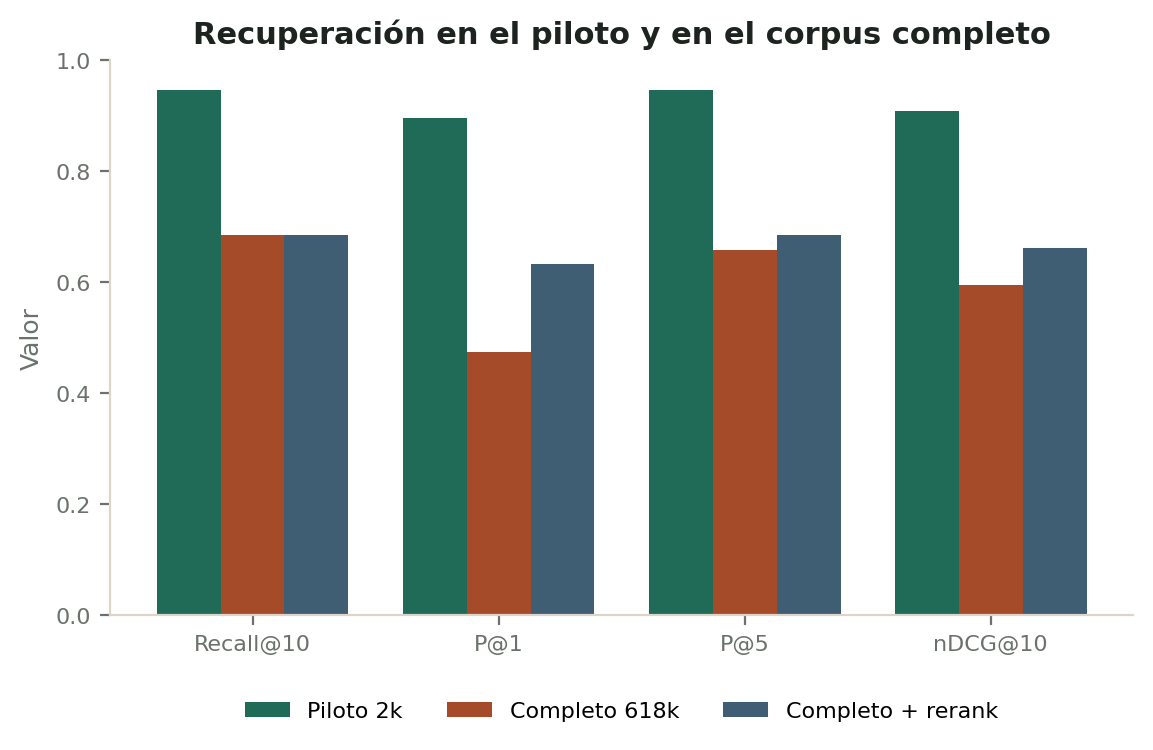
\includegraphics[width=0.85\textwidth]{escala_e6_e7.png}
\caption{Recuperación en el piloto y en el corpus completo, con y sin reranking.}
\label{fig:escala}
\end{figure}

Con 85 veces más candidatos, el mismo codificador y el mismo índice pierden 26 puntos de Recall@10 y 31 de nDCG@10. La latencia no cambia: 42 ms en el corpus completo contra 40 ms en el piloto. El costo es de calidad, no de velocidad. Los documentos de referencia siguen en la colección, así que el problema es de ranking y no de datos faltantes.

Este es el hallazgo principal del trabajo y tiene una consecuencia inmediata sobre la interpretación de todo lo anterior: las cifras del piloto no se pueden presentar como resultado final del sistema. Las ablaciones de limpieza, segmentación y $k$ se hicieron sobre 1.932 documentos y sus conclusiones valen para ese régimen. La comparación de modelos generativos también se hizo sobre el piloto y así se declara. El paso siguiente natural es reranking sobre el top-50 o un codificador más fuerte, no aumentar $k$ a ciegas, porque el documento relevante no está en el top-10 en el 31,6\,\% de las preguntas.

\subsection{E7: reranking sobre el corpus completo}

Se aplicó el cross-encoder \texttt{BAAI/bge-reranker-v2-m3} sobre el top-50 de e5, con top-10 final, 38 preguntas respondibles, 3 repeticiones y \texttt{max\_length=512}. La Tabla~\ref{tab:e7} compara con y sin reranking.

\begin{table}[htbp]
\centering
\footnotesize
\begin{tabular}{@{}lrr}
\toprule
Métrica & Sin rerank (E6) & Con rerank (E7) \\
\midrule
Recall@10 & 0,684 & 0,684 \\
P@1 & 0,474 & \textbf{0,632} \\
P@5 & 0,658 & \textbf{0,684} \\
MRR@10 & 0,564 & \textbf{0,654} \\
nDCG@10 & 0,594 & \textbf{0,661} \\
Cobertura de span & 0,684 & 0,684 \\
Recuperación p50 & \textbf{42 ms} & 3.144 ms \\
\bottomrule
\end{tabular}
\caption{E7: efecto del cross-encoder sobre el top-50 en el corpus completo.}
\label{tab:e7}
\end{table}

El reranker mejora el orden: P@1 sube 15,8 puntos, MRR 9,0 y nDCG 6,7. No mejora la cobertura: el 31,6\,\% de las preguntas que no tenían el documento en el top-10 sigue sin tenerlo, porque el cross-encoder solo reordena lo que el recuperador ya trajo. La latencia pasa de 42 ms a 3.144 ms por consulta, y no baja al limitar \texttt{max\_length} a 512: el costo es del cross-encoder de 568 millones de parámetros evaluando 50 pares. Para la demostración se decide no adoptarlo y se deja como mejora documentada. En un sistema con presupuesto de latencia de segundos, la relación costo-beneficio sería distinta.

\subsection{E8: BM25 sparse sobre el corpus completo}
\label{sec:sparse}

BM25 sparse fue el primer recuperador no denso probado. La colección sparse se construyó a partir de los mismos 618.286 chunks, sin recalcular embeddings, y se evaluó con las 38 preguntas respondibles y 3 repeticiones.

\begin{table}[htbp]
\centering
\footnotesize
\begin{tabular}{@{}lrrrrrrr@{}}
\toprule
Método & Recall@10 & P@1 & P@5 & MRR@10 & nDCG@10 & Span & p50 \\
\midrule
Denso e5 & 0,684 & 0,500 & 0,658 & 0,578 & 0,604 & 0,684 & 48 ms \\
BM25 sparse & \textbf{0,763} & \textbf{0,684} & \textbf{0,737} & \textbf{0,715} & \textbf{0,727} & \textbf{0,763} & \textbf{7 ms} \\
\bottomrule
\end{tabular}
\caption{E8: dense contra BM25 sparse sobre el corpus completo, 38 preguntas respondibles.}
\label{tab:e8}
\end{table}

BM25 sube el Recall@10 7,9 puntos, el nDCG 12,3 y el P@1 18,4, y baja la latencia de 48 a 7 ms. La mejora se concentra en el español (Recall de 0,862 a 0,931) y en el inglés (de 0,111 a 0,222). El inglés sigue siendo el límite: 7 de las 9 preguntas no tienen el documento en el top-10.

La fusión dense más BM25 con pesos 0,3/0,7 se probó y no superó a BM25 solo: Recall 0,763, nDCG 0,694 y P@1 0,632, con 56 ms. BM25 se adoptó de forma provisional hasta medir bge-m3 en el corpus completo. El sistema final usa bge-m3 (Sección~\ref{sec:bge}). Un cross-encoder de 278 millones sobre el top-50 sparse tampoco mejoró el orden: nDCG 0,681, P@1 0,605 y 777 ms por consulta.

\subsection{E10: bge-m3 sobre el corpus completo}
\label{sec:bge}

El sistema final usa \path{BAAI/bge-m3} con 1.024 dimensiones. Los 618.286 chunks se reindexaron en \path{rag_full_bge_m3_d1024_v1} reutilizando los chunks existentes, sin re-chunkear, en 27,3 minutos con fp16 en la RX 9070. En fp32 el mismo modelo tarda 11,5 horas; fp16 lo acelera 28 veces y los resultados del piloto son idénticos.

\begin{table}[htbp]
\centering
\footnotesize
\begin{tabular}{@{}lrrrrrr@{}}
\toprule
Método & Recall@10 & P@1 & P@5 & nDCG@10 & Span & p50 \\
\midrule
Denso e5 & 0,684 & 0,500 & 0,658 & 0,604 & 0,684 & 48 ms \\
BM25 sparse & 0,763 & \textbf{0,684} & 0,737 & \textbf{0,727} & \textbf{0,763} & \textbf{7 ms} \\
bge-m3 & \textbf{0,842} & 0,553 & \textbf{0,816} & 0,708 & 0,737 & 56 ms \\
\bottomrule
\end{tabular}
\caption{E10: e5, BM25 sparse y bge-m3 sobre el corpus completo, 38 preguntas respondibles.}
\label{tab:e10}
\end{table}

bge-m3 cumple el objetivo: Recall@10 de 0,842 y nDCG de 0,708. Sube el inglés de 0,111 a 0,667 y el español de 0,862 a 0,897. BM25 conserva mejor P@1 y nDCG, y es ocho veces más rápido, pero su techo de cobertura es 0,763. bge-m3 fue el paso que recuperó la cobertura; la Sección~\ref{sec:ajuste} añade la fusión con BM25. BM25 solo queda como opción de baja latencia con \texttt{RETRIEVER=sparse}.

\subsection{E11: ajuste de ef y fusión final}
\label{sec:ajuste}

Con bge-m3 se probaron dos ajustes que no requieren reindexar: el parámetro \texttt{ef} del índice HNSW y la fusión con BM25 sparse. La Tabla~\ref{tab:e11} resume el resultado.

\begin{table}[htbp]
\centering
\footnotesize
\begin{tabular}{@{}lrrrrrr@{}}
\toprule
Método & Recall@10 & P@1 & P@5 & nDCG@10 & Span & p50 \\
\midrule
Denso ef=200 & 0,868 & 0,553 & 0,842 & 0,725 & 0,789 & 7 ms \\
Denso ef=800 & 0,895 & 0,553 & 0,868 & 0,738 & 0,816 & 13 ms \\
Híbrido 0,5/0,5 ef=800 & \textbf{0,895} & \textbf{0,684} & \textbf{0,895} & \textbf{0,807} & \textbf{0,868} & 19 ms \\
Reranker sobre ef=800 & 0,868 & 0,526 & 0,789 & 0,702 & 0,895 & 792 ms \\
\bottomrule
\end{tabular}
\caption{E11: ajuste de ef y fusión con BM25 sobre bge-m3, 38 preguntas respondibles.}
\label{tab:e11}
\end{table}

\texttt{ef}=800 sube el Recall 2,6 puntos y el nDCG 1,3 con 6 ms más. La fusión 0,5/0,5 empata en Recall y sube nDCG 6,9, P@1 13,2 y cobertura de span 5,3, con 19 ms de búsqueda. El reranker no mejora: baja el nDCG y el P@1 y cuesta 792 ms. Con el gold de un solo relevante la fusión ganaba en orden. La Sección~\ref{sec:ampliado} muestra que con el gold ampliado gana el dense.

\subsection{E12: gold ampliado y configuración final}
\label{sec:ampliado}

Dos anotadores revisaron 76 documentos candidatos, dos por pregunta, recuperados por bge-m3 y fuera del gold original. El acuerdo fue de 0,626 de kappa, con 12 discrepancias. Se añadieron al gold los 17 documentos marcados como relevantes por ambos. Catorce preguntas quedaron con dos o más documentos relevantes.

\begin{table}[htbp]
\centering
\footnotesize
\begin{tabular}{@{}llrrrrr@{}}
\toprule
Método & Gold & Recall@10 & nDCG@10 & P@1 & P@5 & Span \\
\midrule
Denso ef=800 & 38 & 0,895 & 0,738 & 0,553 & 0,868 & 0,816 \\
Híbrido 0,5/0,5 & 38 & 0,895 & 0,807 & 0,684 & 0,895 & 0,868 \\
Denso ef=800 & ampliado & \textbf{0,921} & \textbf{0,827} & \textbf{0,737} & \textbf{0,947} & 0,816 \\
Híbrido 0,5/0,5 & ampliado & 0,890 & 0,804 & \textbf{0,737} & \textbf{0,947} & \textbf{0,868} \\
\bottomrule
\end{tabular}
\caption{E12: dense contra híbrido con el gold original y el ampliado.}
\label{tab:e12}
\end{table}

Con un solo relevante por pregunta la fusión ganaba en orden. Con el gold ampliado, el dense recupera más de los documentos nuevos: Recall@10 0,921 frente a 0,890, y nDCG 0,827 frente a 0,804. El sistema final usa bge-m3 con \texttt{ef}=800 y sin fusión. La cobertura de span no cambia porque los documentos añadidos no tienen span anotado.

\section{Análisis de errores}

\subsection{Errores de recuperación}

En el piloto los dos fallos del gold son g-045 y g-046, y en ambos el documento está en la colección. En el corpus completo el patrón se repite a mayor escala: 12 de las 38 preguntas respondibles no tienen el documento de referencia en el top-10 con el codificador denso, y 6 con bge-m3. Con el gold ampliado y el dense final quedan 3. El análisis siguiente se hizo sobre la corrida densa. El reranking recupera parte del orden pero no esas 12, lo que confirma que el problema está en la etapa de recuperación densa y no en la de ordenamiento. Las causas plausibles son tres: la competencia entre 618.286 chunks hace que documentos con vocabulario genérico suban por encima del específico; el truncamiento del 32,7\,\% de los documentos elimina la frase que responde la pregunta; y el chunking fijo puede partir la evidencia en dos fragmentos que compiten entre sí. El experimento no separa esas causas, y hacerlo exige una ablación por pregunta que queda como trabajo futuro.

\subsection{Conducta de generación}

Los cuatro modelos fallan de formas distintas con la misma evidencia. qwen2.5:1.5b responde sin citar en el 89,5\,\% de los casos: la respuesta puede ser correcta, pero el usuario no puede verificar de dónde sale. llama3.2:3b cita la mitad de las veces, un comportamiento intermedio que no permite confiar en la cita como garantía. llama3.2:1b se abstiene en el 73,7\,\% de las preguntas respondibles, lo que sugiere que el umbral de abstención y el prompt están calibrados para modelos con más capacidad. gemma2:2b cita siempre y responde casi siempre, pero es el único que responde preguntas sin respuesta en 3 de 15 repeticiones, es decir, alucina con evidencia insuficiente.

\subsection{Abstención}

La abstención se evalúa sobre las 5 preguntas sin respuesta del gold, con 3 repeticiones por modelo. Tres modelos se abstienen en las 15 repeticiones; gemma2:2b lo hace en 12. El resultado agregado oculta un problema de diseño: la abstención del sistema ocurre antes de llamar al modelo cuando la mejor puntuación no supera el umbral, pero las 5 preguntas sin respuesta sí recuperan fragmentos con puntuaciones altas, porque el corpus habla de temas parecidos. La decisión de abstener queda entonces en el prompt, que es el eslabón menos fiable con modelos pequeños.

\subsection{Inyección de instrucciones}

La prueba de E5 muestra que dos de los tres modelos ignoran instrucciones explícitas dentro del texto recuperado. gemma2:2b obedeció una de cinco y añadió la palabra pedida a una respuesta por lo demás correcta. El resultado no permite generalizar, pero sí extraer una regla de diseño: el prompt debe delimitar la evidencia y ordenar explícitamente ignorar instrucciones internas, y esa orden debe repetirse después del bloque de contexto, no solo antes.

\subsection{Errores de diseño del protocolo}

El experimento de limpieza se lanzó inicialmente con el gold de humo, que pertenece a una muestra de 600 documentos que no es subconjunto del piloto de 2.000. Las referencias no existían en las colecciones y las métricas habrían sido cero. El error se detectó al medir y obligó a construir un gold específico para el piloto. La lección es que el gold debe declarar explícitamente a qué muestra pertenece y que la ingesta debe verificar que los documentos de referencia estén en la colección antes de evaluar. Esa verificación ahora forma parte del protocolo.

\section{Limitaciones}
\label{sec:limitaciones}

\begin{enumerate}
\item \textbf{Revisión del gold incompleta.} Carlos revisó las 43 filas y Julián revisó 40; Erika y Óscar no revisaron. De las 40, 30 se confirmaron, 8 se corrigieron (7 spans y una pregunta) y 2 se rechazaron sin cambio porque el texto indexado respalda el valor actual. Tres preguntas no se pudieron verificar por enlaces caídos (404). El gold corregido sube la cobertura de span de E6 de 0,658 a 0,684.
\item \textbf{Composición del gold.} No hay preguntas comparativas ni ambiguas, solo 2 preguntas de Bluesky y 9 en inglés. El margen de $k=5$ para preguntas comparativas no se puede validar con este conjunto.
\item \textbf{E4 sobre el piloto.} La comparación de modelos generativos se hizo sobre 1.932 documentos. En el corpus completo la evidencia recuperada es peor, así que la corrección de los cuatro modelos sería menor y el orden entre ellos podría cambiar.
\item \textbf{Anotación humana acotada.} La rúbrica cubre 18 preguntas respondibles del piloto y dos anotadores. La fidelidad no alcanzó acuerdo (kappa 0,12) y no se usa. En el corpus completo la corrección sería menor.
\item \textbf{Costo del reranking.} E7 mejora el orden con 3,1 s por consulta, un costo incompatible con la demostración interactiva. La alternativa de un cross-encoder más pequeño no se midió.
\item \textbf{Truncamiento y ruido del corpus.} El 32,7\,\% de los documentos está truncado y el 5,3\,\% contiene patrones de ruido. El filtro descarta 7.380 documentos y esa pérdida no se puede recuperar.
\item \textbf{Cobertura del servidor de embeddings.} La ruta del servidor se validó con una muestra de 100 textos y con el piloto, no con el corpus completo.
\item \textbf{Precisión acotada.} Con un solo documento relevante por pregunta, la precisión@$k$ está acotada por $1/k$. Las decisiones se toman con Recall, P@1, P@5, MRR y nDCG, y así se declara.
\item \textbf{Una máquina y una corrida por configuración.} Las 3 repeticiones comparten semilla y temperatura 0, así que miden estabilidad del sistema, no variabilidad entre entrenamientos.
\item \textbf{Prueba de inyección pequeña.} Cinco documentos y tres modelos no constituyen un benchmark adversarial.
\end{enumerate}

\section{Conclusiones}

La limpieza conservadora y el chunking fijo son la base estable del sistema. V2 obtiene la mejor estimación puntual en las cuatro métricas de calidad y elimina las páginas de error del crawler, con costo nulo. El chunking fijo de 1.000 caracteres con 150 de solape gana en estimación puntual y es 3,65 ms más rápido que la segmentación por oraciones. Ninguna de las dos decisiones alcanza significancia estadística con 30 preguntas, y así se reporta: son decisiones de ingeniería sostenidas en consistencia y costo, no en superioridad demostrada.

El tamaño del corpus cambia el resultado. Con el mismo codificador, el mismo índice y las mismas preguntas, Recall@10 cae de 0,947 a 0,684 y nDCG@10 de 0,909 a 0,594 al pasar de 1.932 a 161.868 documentos indexados. La latencia se mantiene en 42 ms, de modo que la degradación es de ranking y no de velocidad ni de datos faltantes. La consecuencia metodológica es que un piloto pequeño sirve para verificar que el pipeline funciona, pero no para estimar el desempeño del sistema final.

BM25 sparse recupera parte de la cobertura perdida sin reindexar embeddings: Recall@10 de 0,684 a 0,763, nDCG de 0,604 a 0,727 y P@1 de 0,500 a 0,684, con 7 ms. bge-m3 recupera el resto: Recall@10 de 0,842 y nDCG de 0,708, con una reindexación de 27 minutos en fp16. El ajuste final, ef=800 y fusión 0,5/0,5 con BM25, lleva el Recall@10 a 0,895 y el nDCG a 0,807. Con el gold ampliado, el dense con ef=800 recupera 0,921 y 0,827, y supera a la fusión. El sistema final usa bge-m3 con ef=800 sin fusión. El inglés sube de 0,111 a 0,889 con el dense, pero sigue por debajo del español.

El reranking mejora el orden sin recuperar la cobertura. P@1 sube de 0,474 a 0,632 y nDCG@10 de 0,594 a 0,661, mientras Recall@10 se queda en 0,684. El cross-encoder reordena lo que el recuperador ya trajo, y el 31,6\,\% de las preguntas sin documento en el top-10 sigue igual. Con 3,1 s por consulta, no se adopta para la demostración.

La anotación humana elige gemma2:2b. Con 18 preguntas respondibles y dos anotadores, supera a qwen2.5:1.5b en corrección (+0,50, IC [+0,11; +1,00]) y en citas (+2,67). El kappa de corrección es 0,95, así que la comparación es interpretable; el de fidelidad es 0,12 y ese eje no se usa. La hipótesis H1 se refuta: llama3.2:3b no supera a qwen2.5:1.5b y pierde contra gemma2:2b.

El sistema es reproducible de extremo a extremo: un archivo de Docker Compose, colecciones separadas por configuración, resultados crudos en JSONL y métricas calculadas desde esos archivos. Esa disciplina fue la que permitió detectar la degradación por escala, porque las cifras del piloto y del corpus completo se midieron con el mismo procedimiento y la misma unidad de análisis.

Quedan dos tareas antes de la entrega: completar la revisión del gold con Erika y Óscar, incluida la verificación de las tres preguntas con enlaces caídos, y ensayar la demostración con el stack levantado y los cuatro modelos.

\bibliographystyle{agsm}
\nocite{*}
\bibliography{referencias}

\appendix

\section{Reproducibilidad}

\subsection{Hardware y versiones}

El equipo local tiene un AMD Ryzen 9 5950X de 16 núcleos y 32 hilos, 31 GB de RAM y una AMD Radeon RX 9070 XT de 16 GB con ROCm 7.2.4. El servidor de embeddings es un Fedora 44 con 16 vCPU (Ryzen 7 5800X, 8 núcleos físicos), 62 GB de RAM y una NVIDIA GTX 1080 de 8 GB. Los contenedores usan Python 3.12, Milvus 2.6.6 y PyTorch 2.10.0 con ROCm 7.2.4.

\subsection{Estructura del repositorio}

\begin{verbatim}
TALLER RAG/
  docker-compose.yml        stack completo, perfiles rocm y embeddings
  Dockerfile                API y frontend
  Dockerfile.rocm           ingesta en GPU AMD
  src/rag/                  pipeline, store, chunking, embeddings, API, UI
  src/scripts/              perfilado, ingesta, evaluacion, metricas
  eval/gold/                gold_standard.jsonl (fuente de verdad)
  reports/corridas/         JSONL crudos de cada corrida
  reports/tablas/           metricas, comparaciones pareadas, textometria
  reports/figuras/          figuras del informe
\end{verbatim}

\subsection{Comandos}

\begin{verbatim}
docker compose up -d --build
docker compose exec api python -m src.scripts.profile_corpus
docker compose exec api python -m src.scripts.build_sample --n 2000
docker compose exec api python -m src.scripts.ingest_v2 \
  --sample eval/pilot_docs.parquet \
  --collection rag_pilot_e5base_d768_v2_v1 --drop
docker compose exec api python -m src.scripts.evaluate \
  --mode retrieve --split test --k 10 --reps 3
docker compose exec api python -m src.scripts.metrics \
  --results reports/corridas/ret_test_k10.jsonl
docker compose --profile rocm run --rm -T ingest-rocm \
  python -m src.scripts.ingest_v2 --sample eval/all_docs.parquet \
  --collection rag_full_e5base_d768_v2_v1 --drop --batch-size 128
\end{verbatim}

\subsection{Artefactos}

El gold consolidado es \texttt{eval/gold/gold\_standard.jsonl} y no debe regenerarse, porque se perderían las correcciones aplicadas. Las corridas crudas están en \texttt{reports/corridas/} y las tablas derivadas en \texttt{reports/tablas/}. Las métricas se recalculan desde los JSONL con \texttt{src/scripts/metrics.py}, y las tablas del informe se transcriben de los CSV que produce ese script.

\end{document}
